%%%%%%%%%%%%%%%%%%%%%%%%%%%%%%%%%%%%%%%%%%%%%%%%%%%%%%%%%%%%%%%%%%%%%%%%%%%%%%%%%%%%%%%%%
% CHAPTER 5 - DESIGN
%%%%%%%%%%%%%%%%%%%%%%%%%%%%%%%%%%%%%%%%%%%%%%%%%%%%%%%%%%%%%%%%%%%%%%%%%%%%%%%%%%%%%%%%%
% Richard Boardman PhD Thesis
% Improving Tool Support for Personal Information Management
%%%%%%%%%%%%%%%%%%%%%%%%%%%%%%%%%%%%%%%%%%%%%%%%%%%%%%%%%%%%%%%%%%%%%%%%%%%%%%%%%%%%%%%%%
% Method notes
%%%%%%%%%%%%%%%%%%
%	How strictly to follow Carroll's methodology in terms of strict design rationale
% and claims analysis? Root in strong psyhological findings?
%		Or do I have a weasel? Claims inherent in bog-standard hierarchy?}
% Form of needs/requirements - relate this to evaluation criteria?
%%%%%%%%%%%%%%%%%%%%%%%%%%%%%%%%%%%%%%%%%%%%%%%%%%%%%%%%%%%%%%%%%%%%%%%%%%%%%%%%%%%%%%%%%
% DESIGN THEORY: need to take care!
% 	TOPLACE: \section{Design as Research} \label{design:design-as-research}
% 	Consider placement of role of design in HCI research here}
%	Relate to nature of design -- purposeful/creative, ITERATIVE, unbounded/never-ending}
%%%%%%%%%%%%%%%%%%%%%%%%%%%%%%%%%%%%%%%%%%%%%%%%%%%%%%%%%%%%%%%%%%%%%%%%%%%%%%%%%%%%%%%%%
%	REMEMBER ANGELA'S CLIFF!
%%%%%%%%%%%%%%%%%%%%%%%%%%%%%%%%%%%%%%%%%%%%%%%%%%%%%%%%%%%%%%%%%%%%%%%%%%%%%%%%%%%%%%%%%
% Need for definitions: PIM tool/software/application
% vs. cross-tool/means of integration/integrating mechanism 
%%%%%%%%%%%%%%%%%%%%%%%%%%%%%%%%%%%%%%%%%%%%%%%%%%%%%%%%%%%%%%%%%%%%%%%%%%%%%%%%%%%%%%%%%
% WORDS
% design rationale/justification/defense
% leverage, motivate, exploit
% strawman/test-bed/research-vehicle
%%%%%%%%%%%%%%%%%%%%%%%%%%%%%%%%%%%%%%%%%%%%%%%%%%%%%%%%%%%%%%%%%%%%%%%%%%%%%%%%%%%%%%%%%
% Key aspects of chapter:
% Following design-science paradigm
% Exploration in cross-tool design space
% Decision to focus on one design
% Communicate how the design came into being
%%%%%%%%%%%%%%%%%%%%%%%%%%%%%%%%%%%%%%%%%%%%%%%%%%%%%%%%%%%%%%%%%%%%%%%%%%%%%%%%%%%%%%%%%
%	Ways of improving support for PIM:
% 	(1) improve support
%		(2) change user practice
% 	(3) dovetailing of the two}
%%%%%%%%%%%%%%%%%%%%%%%%%%%%%%%%%%%%%%%%%%%%%%%%%%%%%%%%%%%%%%%%%%%%%%%%%%%%%%%%%%%%%%%%%


%%%%%%%%%%%%%%%%%%%%%%%%%%%%%%%%%%
\section{Introduction}
\label{design:introduction}
%%%%%%%%%%%%%%%%%%%%%%%%%%%%%%%%%%

%%%%%%%%%%%%%%%%%%%%%%%%%%%%%%%%%%%%%%%%%%%
% General intro
%		Relate to overall PhD aims
% Perspective to mention: Continued operationalization of cross-tool
% research methodology outlined in \textbf{Chapter~\ref{chapter:research_agenda}}, 
%%%%%%%%%%%%%%%%%%%%%%%%%%%%%%%%%%%%%%%%%%%
This chapter reports the design, implementation, and initial evaluation of the \textit{WorkspaceMirror} prototype, abbreviated to WM henceforth.  WM provides a novel integration mechanism between three collections of personal information (files, email and bookmarks) based on the principle of \textit{folder mirroring} -- the sharing of organizational structure across PIM-tools.


%%%%%%%%%%%%%%
% DESIGN AIMS
%%%%%%%%%%%%%%
%%%%%%%%%%%%%%%%%%%%%%%
% METHOD/CROSS-TOOL
%%%%%%%%%%%%%%%%%%%%%%%
% Explore how to design along cross-tool dimension. Driving concern: operationalize  cross-tool principles in terms of design recommendations -- making cross-tool perspective ``operationalizable''
% \item \textit{Focus on one novel \textit{cross-tool} support for PIM -- i.e. creation of an artefact that embodies implicit psychological claims.}
%%%%%%%%%%%%%%%%%%%%%%%%%
% Method: Form of design objectives
%%%%%%%%%%%%%%%%%%%%%%%%%%%%%%%%%%%%%%%%%
%%%%%%%%%%%%%%%%%%%%%%%%%%%%%%%%%%
% Design philosophy/perspective
% * must use these to drive aims or vice versa
% motivating factors
% specify Design Theory and Approaches influencing my work?
%%%%%%%%%%%%%%%%%%%%%%%%%%%%%%%%%%
% Design perspective (driven by critique of previous design/technology and my own cross-tool perspective:):
%%%%%%%%%%%%%%%%%%%%%%%%
% Previous work:
% %%%%%%%%%%%%%%%
% lack of empirical motivation
% complex. Aimed at techies?
% revolutionary.  Therefore hard to learn, implement, evaluate.
% Lack of evaluation.  Therefore bottom line: little contribution to knowledge
%%%%%%%%%%%%%%%%%%%%%%%%%%%%%%%%%%%%%%
% ADD: Discuss in terms of T/A cycle
%%%%%%%%%%%%%%%%%%%%%%%%%%%%%%%%%%%%%%
% Desire to complete the cycle THINK: MOVE EARLIER Base on Carroll and Rosson's Task-Artefact Theory - artefact as theory. Task provides requirements for artefact, AND artefact redefines/provides new possibilities for the task.
%%%%%%%%%%%%%%%%%%%%%%%%%%%%%%%%%%%%%%%%%%%%%%%%%%%%%%%%%%%%%%%%%%%%%%%%%%%%%%%%
% ADD: Cross-tool perspective
% Each objective entails building on the limitations of previous design work in this area
% As well as these overall objectives, a key consideration was to improve upon the limitations of previous PIM prototypes as highlighted in the literature review (\textbf{Chapter~\ref{chapter:review}}).
% These are discussed as follows. % UPDATE SECTION NUMBER
%%%%%%%%%%%%%%%%%%%%%%%%%%%%%%%%%%%%%%%%%%%%%%%%%%%%%%%%%%%%%%%%%%%%%%%%%%%%%%%%
%Rooted in cross-tool perspective (i.e. principled)
%\begin{itemize}
%		\item Perspective as design principled approach
%		\item Focus here: improve integration/consistency/unification between PIM tools that make up the personal digital workspace. Focus: storage/organization.
%		\item Cross-tool solutions to cross-tool problems
%		\item \textit{THINK: integration between tools or between activities}
%%%%%%%%%%%%%%%%%%%%%%%%%%%%%%%%%%%%%%%%%%%%%%%%%%%%%%%%%%%%%%%%%%%%%%%%%%%%%%%%
\subsection{Aims}
\label{design:aims}
%%%%%%%%%%%%%%%%%%%%%%%%%%%%%%%%%%%%%%%%%
% This section presents the objectives of the design work, and the design approach that was taken.
The design component of this thesis had three high-level objectives, each relating to a limitation of previous design work in this area:
\begin{enumerate}

%%%%%%%%%%%%%%%%%%%%%%%%%%%%%%%%%%%%%%%%%
% DESIGN TOOL WITH Empirical grounding
%%%%%%%%%%%%%%%%%%%%%%%%%%%%%%%%%%%%%%%%%
% Basis in problems observed in exploratory study. Grounded in empirical evidence. lack of empirical motivation
% The design rationale must be grounded in empirical data
% A second key criticism that can be levelled at many previous prototypes is that they have not been grounded in empirical data, but rather founded on  (see ).  \citet{Carroll:00} discusses the importance of empirical grounding.  
% The design should be grounded in findings from the exploratory study.
%  --  (i.e. answer the design question: how can integration between existing PIM tools be enhanced to better support user needs?) 
\item \textit{To propose a design that offers a new form PIM integration to better meet user needs} -- \textbf{Chapter~\ref{chapter:review}} criticises a number of previous research prototypes in this area for a lack of empirical grounding.  Instead, many have been founded on designer intuition.  To avoid similar criticism, the author set out to ground his design efforts in findings from \textbf{Chapter~\ref{chapter:exploratory_study}}.

\item \textit{To implement the design with an aim of performing a long-term evaluation} -- This was to counter a second limitation of previous prototypes: that in most cases they have not been evaluated to test designers' claims.  Therefore, any implementation had to be sufficiently robust to sustain long-term usage in real-world conditions.  
%  to:  (1) explore issues related to improving integration between PIM tools; and (2) develop appropriate methodology for evaluating PIM tools.

\end{enumerate}

%%%%%%%%%%%%%%%%%%%%%%%%%%%%%%%
\subsection{Design Approach}
%%%%%%%%%%%%%%%%%%%%%%%%%%%%%%%
%%%%%%%%%%%%%%%%%%%%%%%%%%
% incremental approach
%%%%%%%%%%%%%%%%%%%%%%%%%%
% Move away from radical invention towards evolutionary, incremental design, measured step.
% This stance is contrasted with that taken by more ambitious ``PIM-unifying'' systems that have been proposed in the past.
% Best chance to complete the cycle
% Don't cross the streams!
% summarized in \textbf{Chapter~\ref{chapter:review}} has produced inventive \textit{revolutionary} designs which offer an alternative to current tools. Although innovative, such designs may offer a barrier to successful uptake and evaluation.
%%%%%%%%%%%%%%%%%%%%%%%%%
% Extra Carroll depth
%%%%%%%%%%%%%%%%%%%%%%%%%
% Have to correctly relate incremental, hill-climbing and cumulative
% Carroll proposes three modes of design reasoning that enable cumulative design, along with their positive and negative aspects: (1) \textit{hill-climbing}, (2) \textit{principled emulation}, and (3) \textit{activity modelling}.
% The second paradigm, principled emulation involves applying designs from other domains. The third paradigm, activity modelling is based on the study of user practices. % TODO: expand on this
% Furthermore, revolutionary design is hard to build on, and \textbf{Chapter~\ref{chapter:review}} observes how the products of such design tend to complex and hard to evaluate.
In contrast to most previous work in this area, the design reported here was deliberately \textit{incremental} -- aimed at extending, rather than replacing existing technology.  This relates to a third criticism of previous work made in \textbf{Chapter~\ref{chapter:review}}: that there has been an over-focus on \textit{revolutionary design}, the innovation of radical alternatives to current tools.  Although many interesting designs have been proposed, such \textit{radical invention} does not necessarily entail a strong contribution in terms of HCI knowledge, especially if no evaluation has been performed.  
In response, a number of researchers have emphasized the need for an iterative, incremental process of design~\citep{ml:88,newman:95,Whittaker-rta:00,Carroll:00}.  This approach has been termed cumulative design, or ``hill climbing''~\citep{Carroll:00}.  In the context of this thesis, an incremental approach was chosen for the following reasons:
\begin{enumerate}

%%%%%%%%%%%%%%%%%%%%%%%%%%%
% Import of evaluation.
%%%%%%%%%%%%%%%%%%%%%%%%%%%
% Facilitate thorough evaluation
% Thus although a range of exciting techniques have been proposed it is difficult 
% third benefit of incremental design is that it facilitates systematic evaluation~.  By making limited changes to the existing personal information environment, it was envisaged that it would be easier to associate specific changes with the design intervention. 
\item \textit{To enable effective evaluation} -- As noted above, a key aim of the work reported in this chapter was to enable effective evaluation.  One downside of radical invention is that it is difficult to measure specific improvements as so many interface aspects may change~\citep{Carroll:00}.  \citet{newman:95} argue that incremental, localized changes that are well-understood and result in subtle improvements, are to be preferred over more ambitious changes which may result in complex side effects.  

%%%%%%%%%%%%%%%%%%%%%%%%%%%%%%%%%%%%%%%%%%%%
% Familiar concepts - promote learnability
%%%%%%%%%%%%%%%%%%%%%%%%%%%%%%%%%%%%%%%%%%%%
%  it was hoped that ease of use would be promoted.
% To promote learnability/user familiarity. 
% incremental changes to retain familiarity - not asking users to start from fresh)
\item \textit{To promote user familiarity} --  By basing design on existing technology, it was envisaged that the likelihood of system uptake would be increased.  Employing familiar concepts and tools will mean that users have less to learn~\citep{Carroll:00}.

%%%%%%%%%%%%%%%%%%%%%%%%%%%%%%%%%%%%%%%%%%%%%%%%%%%%%%%%%%%%%%%%%
% easier bootstrapping - Supports aim for long-term evaluation. 
%%%%%%%%%%%%%%%%%%%%%%%%%%%%%%%%%%%%%%%%%%%%%%%%%%%%%%%%%%%%%%%%%
% prime aim was to ensure compatibility with the existing personal information environment.  
% bootstrapping and minimize disruption to the user
\item \textit{To promote system up-take} -- Building on current tools implicitly encourages compatibility with previous data formats.  It was envisaged that this would make long-term evaluation more straightforward, since a tool that can be easily integrated into a user's existing tool-set is more likely to be used.  % In addition, at the end of the evaluation, it was intended that the prototype could be easily removed with minimal impact.
A major concern was to avoid prospective users having to go through complex data-import processes, or abandon carefully nurtured collections of personal information in favour of an unproven technology.  

%%%%%%%%%%%%%%%%
% Achievable
%%%%%%%%%%%%%%%
% influence of external constraints/pragmatics on choice of method}
\item \textit{To encourage an achievable design goal} -- Another key concern was that the design and implementation needed to be achievable in the context of the limited time and man-power resources available. An incremental approach allowed the author to build on previous design expertise manifested in already available tools.

\end{enumerate}

%%%%%%%%%%%%
% DOWNSIDE
%%%%%%%%%%%%
% also argues in favour of incremental design (also known as cumulative design or ``hill climbing''). He discusses how this approach offers familiarity for users, and the benefits of grounding in previous design expertise.  However, he also observes potential downsides including the possibility of inheriting from poor previous designs, and the limitations to local optimization. 
\citet{Carroll:00} observes a fundamental limitation of incremental design.  Along with the benefits of building on previous design expertise comes the risk of inheriting previous design limitations.  Therefore, the designer may be constrained to making little more than local optimizations.
%%%%%%%%%%%%%%%%%%%%%%%%%%%%%%
% Can change later anyway
%%%%%%%%%%%%%%%%%%%%%%%%%%%%%%
% Additional functionality can be added based on initial evaluation results.
However, it is observed that an incremental design approach facilitates subsequent iterative refinement once initial changes have been evaluated.  In other words, following an incremental strategy does not mean that further more ambitious changes cannot be made. 

%%%%%%%%
% UCD
%%%%%%%%
%%%%%%%%%%%%%%%%%%%%%%%%%%%%%%%%%%%%%%%%%%%%%%%%%%%%%%%%%%%%%%%%%%%%%%%%%%%%
\subsection{Structure of the Chapter}
%%%%%%%%%%%%%%%%%%%%%%%%%%%%%%%%%%%%%%%%%%%%%%%%%%%%%%%%%%%%%%%%%%%%%%%%%%%%
% Adopt \textbf{standard usability engineering-style loop} (Dix, Preece, Whiteside, Nielsen) -- \textit{iterative prototyping and evaluation of usability is key}, (cf. User-centred Design (Norman and Draper), Scenario-based Design~\citep{Carroll:00}, yeartest~\citen{Carroll:00}.
%%%%%%%%%%%%%%%%%%%%%%%%%%%%%%%%%%%%%%%%%%%%%%%%%%%%%%%%%%%%%%%%%%%%%%%%%%%%
% Method: Description of design method (can I claim participatory design?)
% This is a mismatch of method, design rationale, and desired characteristics of target design
%%%%%%%%%%%%%%%%%%%%%%%%%%%%%%%%%%%%%%%%%%%%%%%%%%%%%%%%%%%%%%%%%%%%%%%%%%%%
% The design methodology followed by the candidate is summarized:
% Design work was carried out as follows.
%%%%%%%%%%%%%%%%%%%%%%%%%%
% Analysis of problems -> initial design space
%%%%%%%%%%%%%%%%%%%%%%%%%%
% Analysis of key problems highlighted in exploratory study (workspace-wide problems)
% Staking out Cross-tool Requirements.
% Initially outline potential design space opened up by findings from the exploratory study. Not Small tool-centric problem in many places/Larger problem that bridges tool. 
% BRAINSTORMING
This chapter reports how an incremental perspective was employed within a user-centred design process.
The first step of the design work was to brainstorm improvements to address user problems identified in the exploratory study reported in \textbf{Chapter~\ref{chapter:exploratory_study}}.  Since a key aim was to investigate routes for improving integration between PIM-tools,  a focus was taken on the problems in \textbf{Section~\ref{exp-study:comparison-problems}} that bridged multiple PIM-tool contexts. 
% INITIAL DESIGN SPACE
% , and associated empirical and theoretical design rationale.
% A range of paper and working prototypes were developed, and assessed by the author.
% Several users asked for feedback
% \textbf{Section~\ref{design:initial-forays}} describes this initial cross-tool design space of problems, and potential solutions.
\textbf{Section~\ref{design:initial-forays}} presents two design avenues which emerged from the exploratory study findings.
% DESIGN FOCUS
% Focus on design ideas that offer increased integration between PIM tools
% One particular idea/design idea to be focused on.
% Consider design trade-off's and consequences
% Making design rationale explicit. \textbf{Design Rationale} techniques to record decisions made in design process and context of those decisions (design space, process-oriented, psychological claims)
Due to time constraints, the thesis focused on one of the candidate design routes, that of \textit{folder-mirroring}. The rationale behind this design focus is presented in \textbf{Section~\ref{design:sharing-mirroring}}, along with a description of the design. %, along with a description of how the design evolved over time. The design rationale behind key decisions is also described, along with open issues that remained before implementation.
% IMPLEMENTATION
\textbf{Section~\ref{design:wm-prototyping}} reports the development of a folder-mirroring prototype, called \textit{WorkspaceMirror} (WM).
% initial evaluation
\textbf{Section~\ref{design:feasibility-study}} then presents an initial evaluation that was carried out to assess the viability of the folder-mirroring principle.  
% COMPARISON compares the principle of folder-mirroring with other approaches to PIM-integration.
Finally, \textbf{Section~\ref{design:discussion}} contrasts WM with other research prototypes.
% \textbf{Section~\ref{design:design-extensions}} details possible design extensions to the core functionality. 

%%%%%%%%%%%%%%%%%%
\subsection{Contributions}
%%%%%%%%%%%%%%%%%%
% Focus on novel cross-tool design of WorkspaceMirror as a major deliverable. As a straw-man to investigate potential to unify PIM support. Incremental design.
% This chapter's main contribution is the design and implementation of WM.
% As well as being an instance of one possible form of PIM-integration, WM is proposed as a research vehicle to enable the investigation of issues relating to PIM-integration.
This chapter makes two main contributions to the thesis:
\begin{enumerate}
\item \textit{The design and implementation of the WM prototype} --  As well as being a novel PIM-integration mechanism, WM acted as a research vehicle to enable the investigation of general issues relating to PIM-integration.
\item \textit{The results from the initial formative evaluation of WM} -- These results confirmed the worth of pursuing a more in-depth evaluation. \textbf{Chapter~\ref{chapter:main-study}} reports a follow-up longitudinal evaluation of a modified version of WM which incorporated suggestions from the initial evaluation.
\end{enumerate}

%%%%%%%%%%%%%%%%%%%%%%%%%%%%%%%%%%%%%%%%%%%%%
% relate to other chapters: past and future
%%%%%%%%%%%%%%%%%%%%%%%%%%%%%%%%%%%%%%%%%%%%%
% The design was motivated by conclusions from the literature review in \textbf{Chapter~\ref{chapter:review}}, along with findings from the exploratory study in \textbf{Chapter~\ref{chapter:exploratory_study}}. % The next chapter, \textbf{Chapter~\ref{chapter:main-study}} describes the longitudinal formative evaluation of WM.


%%%%%%%%%%%%%%%%%%%%%%%%%%%%%%%%%%%%%%%%%%%
% \subsection{Structure of the Chapter}
%%%%%%%%%%%%%%%%%%%%%%%%%%%%%%%%%%%%%%%%%%%
%%%%%%%%%%%%%%%%
% Structure
%%%%%%%%%%%%%%%%
% The chapter is structured as follows.
% Firstly, \textbf{Section~\ref{design:aims}} discusses design aims and approach. 
% \textbf{Section~\ref{design:sharing-mirroring}} discusses the focus that was taken on one of these: \textit{folder-mirroring}. \textbf{Section~\ref{design:comparison}} compares folder-mirroring with related prototypes to date.
%  \textit{folder-sharing}, and details a particular approach to folder-sharing, . % specialization?
% Next, \textbf{Section~\ref{design:wm-prototyping}} describes the implementation of WM based on the folder-mirroring principle. \textbf{Section~\ref{design:feasibility-study}} reports an initial field trial of WM to assess its viability.  Finally, \textbf{Section~\ref{design:summary}} summarises the work presented in the chapter and discusses the contributions made.  This section also proposes the theoretical concept of a cross-tool artefact, and discusses consequent methodological considerations for the evaluation of such an artefact.
%  that lead from the cross-tool design work presented in this chapter.
% which were taken into account during the evaluation work reported in \textbf{Chapter~\ref{chapter:main_study}}.

%%%%%%%%%%%%%%%%%%%%%%%%%%%%%%%%%%%%%%%%%%%%%%%%%%%%%%%%%%%%%%%%%%%%%%%%%%%%%%%%%%
%%%%%%%%%%%%%%%%%%%%%%%%%%%%%%%%%%%%%%%%%%%%%%%%%%%%%%%%%%%%%%%%%%%%%%%%%%%%%%%%%%
%%%%%%%%%%%%%%%%%%%%%%%%%%%%%%%%%%%%%%%%%%%%%%%%%%%%%%%%%%%%%%%%%%%%%%%%%%%%%%%%%%
%%%%%%%%%%%%%%%%%%%%%%%%%%%%%%%%%%%%%%%%%%%%%%%%%%%%%%%%%%%%%%%%%%%%%%%%%%%%%%%%%%

%%%%%%%%%%%%%%%%%%%%%%%%%%%%%%%%%%%%%%%%%%%%%%%%
%%%%%%%%%%%%%%%%%%%%%%%%%%%%%%%%%%%%%%%%%%%%%%%%
\newpage
\section{Initial Forays in a Cross-tool Design Space}
% \section{Staking out the cross-tool design space}
\label{design:initial-forays}
%%%%%%%%%%%%%%%%%%%%%%%%%%%%%%%%%%%%%%%%%%%%%%%%
% THINK: Present design rationale in the form of claims? (upsides/downsides)}
% Can I avoid "creative leap" syndrome?
% Method: Form of design rationale in describing design
% Cover all envisaged designs, or just WorkspaceMirror?
% Wording: Potential designs. candidate designs
%%%%%%%%%%%%%%%%%%%%%%%%%%%%%%%%%%%%%%%%%%%%%%%%

%%%%%%%%%%%%%%%%%%%%%%%%%%%%%%%%%%
% 2 types of cross-tool problem
% 1. within-tool -- intra tool, consistent
% 2. cross-tool -- need for coordination
%%%%%%%%%%%%%%%%%%%%%%%%%%%%%%%%%%
% Informed by data from the exploratory study, an initial design space was developed by the author. Potential routes for design work are identified, motivated by specific findings from the exploratory study, and discussed in terms of the conceptual framework outlined in Chapter 5. The considered design routes are discussed (see \textbf{Figure~\ref{fig:design:initial_designs}}):
% Initial prototyping carried out to explore the viability of each design is described.
%Discuss the following for each:
%\begin{itemize}	
%		\item Motivating results from exploratory study.
%			\item their design rationale, synthesis of ideas and theories influencing design. 
%			\item support for design decisions made (TA, LR, CTF, ES)
%			\item inherent trade-off's, balance arguments for and against
%			\item What aspects of PIM are they supporting?
%			\item How they fit into cross-tool analytical framework
%			\item Comment on generality across users, severity of problem they're solving
%			\item i.e. generally add more detail with DIAGRAMS for each
%\end{itemize}
% ADD: provide scenarios for each?
% ADD compare to related research?

%%%%%%%%%%%%%%%%%%%%%%%%%%%%%%%%%%%%%%%%%%%%%%%
% The following designs emerged from the data
%%%%%%%%%%%%%%%%%%%%%%%%%%%%%%%%%%%%%%%%%%%%%%%
% \textit{Two types of cross-tool problem were identified in \textbf{Chapter~\ref{chapter:exploratory_study}}: (1) within-tool problems that occur in multiple tool contexts (e.g. ADD EXAMPLE), and (2) cross-tool problems that bridge multiple tools (e.g. ADD EXAMPLE).}
% This section surveys the initial design space that emerged from the exploratory study findings.  The findings reported in \textbf{Chapter~\ref{chapter:exploratory_study}} included several sets of user needs which corresponded with potential routes for improved design integration.  In this section, two sets of cross-tool problems are described, along with the initial design prototyping carried out by the author. Each problem involves multiple PIM-tools.
This section reports initial incremental design and prototyping directed at solving two of the \textit{cross-tool} problems identified in \textbf{Section~\ref{exp-study:comparison-problems}}.  Note that both are incremental adjustments to commonly available PIM-tools.

% The first concerns the use of different types of information as reminders.  The second relates to the need to organize different types of information in separate folder structures.

%%%%%%%%%%%%
% Naming
%%%%%%%%%%%%
% provide an enhanced naming mechanism, consistent across all PIM tools. Motivation by user problems relating to naming items.
% QUESTION: are there any quotes I can add? \textbf{QUOTES}
%%%%%%%%%%%%%%%%%%%%%%%%%%%
% \subsection{Naming items}
%%%%%%%%%%%%%%%%%%%%%%%%%%%
% Several participants complained of difficulties naming items of information in various tools.  In particular, the naming of bookmarks was seen as unsatisfactory by several participants.  They complained that the default name assigned to new bookmarks (that of the title meta-data from the page they pointed to) were often inappropriate.  Furthermore, changing the name from the default setting was seen as clumsy. For instance, using some content from within the page to name the newly created bookmark involved a laborious process of selecting the bookmark, and then copying and pasting the text.  One participant complained that it was not easily possible to rename email subjects.  The naming problem space can be considered cross-tool in the sense that participants encountered difficulties within multiple PIM-tools. Participants complained of the lack of consistency between PIM-tools regarding functionality such as naming items. 
% A new mechanism was developed by the author to make it easier to name bookmarks with arbitrary content from the referenced web page, termed \textit{in-line naming}.  Instead of creating the bookmark and then renaming it, the user can first select some text on a web-page, and then via a context-menu, specify that text as the name of a new bookmark referencing that page.  A working prototype was developed by the author in the context of MS-Internet Explorer.  Furthermore, the lack of consistency between tools in terms of naming functionality could be addressed by offering in-line naming and renaming of items across all PIM-tools.
% based on the \textit{Consistent Naming Principle}: users should have a consistent mechanism for naming an item in all PIM-tools, be it a file, email or bookmark.  The envisaged design allowed the user to select any arbitrary text in an item, and via .  


%%%%%%%%%%%%%%%%%%%%%%%%%%%%%%%%%%
% Todo highlighting + groupable
%%%%%%%%%%%%%%%%%%%%%%%%%%%%%%%%%%%%%%%%%%%%%%%%%%%%%
\subsection{Highlighting and Gathering To-do Items}
%%%%%%%%%%%%%%%%%%%%%%%%%%%%%%%%%%%%%%%%%%%%%%%%%%%%%

Several participants in the exploratory study mentioned problems relating to the use of information as reminders.  These included a lack of consistency between different tools regarding support offered for highlighting an item as a \textit{to-do item}. A second problem was that it was hard to gather together to-do items from different tools.
% For instance, MS-Outlook allows the ``flagging'' of messages within the email view. However, the Windows file manager and MS-Internet Explorer do not offer any similar functionality.  A second problem reported by a number of participants was that it was hard to gather together related items, such as to-do items. % Note that no participants made use of dedicated to-do managers, such as the ``Tasks view'' in MS-Outlook 

% MOVE TO CHAPTER 4?
The author's proposed solution allowed any item of information to be highlighted and marked as a to-do.  To-do items are highlighted in a consistent manner across all tools via a standardized context-menu mechanism.  At the same time, a reference to each new to-do item is added to a unified list.  An initial proof-of-concept was developed on MS-Windows using MS-Visual Basic 6.0, allowing any desktop icon, file, or bookmark, to be selected and highlighted as a to-do.  This resulted in the icon background changing to red. A short-cut to the item was also added to the MS-Outlook ``tasks view''.  However, it was not possible to provide the same mechanism for highlighting emails due to imitations on the MS-Outlook object model.  This design can be related to the functionality present in attribute-based systems that allow users to label arbitrary pieces of personal information with an attribute such as ``to-do'' or ``important'', e.g.\citep{dourish:99a}.  The author's work can be differentiated due to the incremental design stance of providing functionality on top of standard PIM-tools.
% Several participants observed the lack of consistency between PIM-tools regarding support offered for highlighting an item as a \textit{to-do}.  For instance, MS-Outlook allows the ``flagging'' of messages within the email view, or the management of a separate list of to-do items in the ``Tasks view''.  Emails or files can be dragged into the separate to-do list. However, the to-do item is not highlighted in its original context and is treated as a separate entity, \textit{P22: ``You sit and look at your inbox - and you have to type or write the to-do item separately, and you can't very easily make an email a to-do item. It involves something that I regard ... a redundant transformation. You know basically converting one form of data into another which doesn't add anything. You know there's no added value there - you don't have any easy way of pushing data from one tool to another, copying it from one space to another''}. % and are embedded within new to-do items.



%%%%%%%%%%%%%%%%%%%%%%%%%%%%%%%%
% Add initial user feedback?
%%%%%%%%%%%%%%%%%%%%%%%%%%%%%%%%

%%%%%%%%%%%%%%%%%%%%
% ADD MORE DETAIL HERE?
% REASONS FOR FOCUS
% \textit{The rationale for focusing on the folder-mirroring is discussed.  }
%%%%%%%%%%%%%%%%%%%%%%%%%%%%%%%%%%%
\subsection{Managing Multiple Types of Information in Parallel}
%%%%%%%%%%%%%%%%%%%%%%%%%%%%%%%%%%%

A second area of difficulty reported by users related to the need to manage distinct collections of personal information across a range of PIM-tools, each with a distinct organizational structure.
%%%%%%%%%%%%%%%%%%%%%%%%%%%%%%
% Various options available
%%%%%%%%%%%%%%%%%%%%%%%%%%%%%%
% The design-space relating to different ways of sharing folder structure is outlined. 
After initial brainstorming, two possible approaches were identified to make it easier for users organize information in multiple PIM-tools:
\begin{enumerate}

%%%%%%%%%%%%%%%%%%%%%%%%%%%%%%%%%%%%%
% More ambitious: folder sharing
%%%%%%%%%%%%%%%%%%%%%%%%%%%%%%%%%%%%%
% cite Presto?
% think generalize `folder' to `container'
% The more ambitious approach to folder-sharing involves \textit{unified storage}. 
\item \textit{Folder sharing} -- This would allow the storage of multiple types of information (e.g. files and email) within a consolidated folder structure.  Two key problems were identified with this route. First, it was not clear how such a scheme would co-exist with current tools, and whether users would employ it in preference to those tools.  Secondly, an initial investigation of the technical feasibility of folder-sharing on MS-Windows, concluded that it was beyond the time and manpower resources of a single PhD researcher.
% In other words the same physical storage would be accessed via multiple PIM-tools.  Two key problems were identified with this route: (1) barriers to usage, and (2) ease of implementation.  First, it was not clear how such a scheme would co-exist with current tools. A prime aim was to carry out the long-term evaluation of a designed artefact.  For this to happen it was seen to be essential that the tool integrated smoothly with existing tools, and did not necessitate the user having to abandon previous collections.  Secondly, an initial investigation of the technical feasibility of folder-sharing on MS-Windows, concluded that it was non-trivial, and would necessitate the building of a substantial new technology.

%%%%%%%%%%%%%%%%%%%%%%%%%%%%%%%%%%%%%%%%%%%%%
% More ambitious: folder mirroring
%%%%%%%%%%%%%%%%%%%%%%%%%%%%%%%%%%%%%%%%%%%%%
\item \textit{Folder-mirroring} --  Rather than storing multiple types of information within the same unified storage, this alternative design allows folder names and their structure to be shared between PIM tools.  However, distinct folder structures are retained in different PIM-tools such as files and email.
% folder-mirroring retains distinct folder structures in different PIM-tools such as files and email.  Only the folder names and folder structure is shared between PIM-tools. 
% allows the user to store each type of information within distinct folders within each collection, sharing the same name. 

\end{enumerate}

% These design options are now discussed, and contrasted in terms of various perspectives including ease of implementation:
% for sharing folders between PIM-tools (see ). 
\textbf{Figure~\ref{fig:design:fs-fm-comparison}} compares these two approaches.
%%%%%%%%%%%%%%%%%%%%%%%%%%%%%%%%%%%%%%%%%%%%%%%%%%%%%%%%%%%%%%%%%%%%%%
% Selection of folder-mirroring based on ease of implementation
% Carefully differentiate f-m from f-s
% state that less ambiitous?
%%%%%%%%%%%%%%%%%%%%%%%%%%%%%%%%%%%%%%%%%%%%%%%%%%%%%%%%%%%%%%%%%%%%%%
% and is discussed in more detail in the next section.  
% Folder-mirroring was selected due to concern over whether users needed some flexibility to manage different types of information in different ways.  In addition, it was seen to be more achievable technically.
% The second potential design, folder-mirroring, addressed issues regarding the compartmentalization of personal information across multiple PIM-tools, each with a distinct organizational structure.  The envisaged design allowed a user to share organizational structure across PIM tools.
% Folder-mirroring was selected as the focus for the thesis for two reasons: (1) stronger empirical grounding, and (2) more progress with initial prototyping.  
The second approach, \textit{folder-mirroring}, was selected as the focus for the thesis, for two reasons: (1) stronger empirical grounding, and (2) more straightforward implementation.  The rest of \textbf{Chapter~\ref{chapter:design}} details the empirical and technological design rationale, implementation, and initial evaluation of a folder-mirroring prototype.
% are discussed in more detail in the next section.

% %%%%%%%%%%%%%%%%%%%%%%%%%%%%%
% FIGURE - Comparison of folder-sharing and folder-mirroring
% %%%%%%%%%%%%%%%%%%%%%%%%%%%%%
%%%%%%%%%%%%%%%%%%%%%%%%%%%%%%
\begin{figure}[htbp]
	\begin{center}
		\leavevmode
		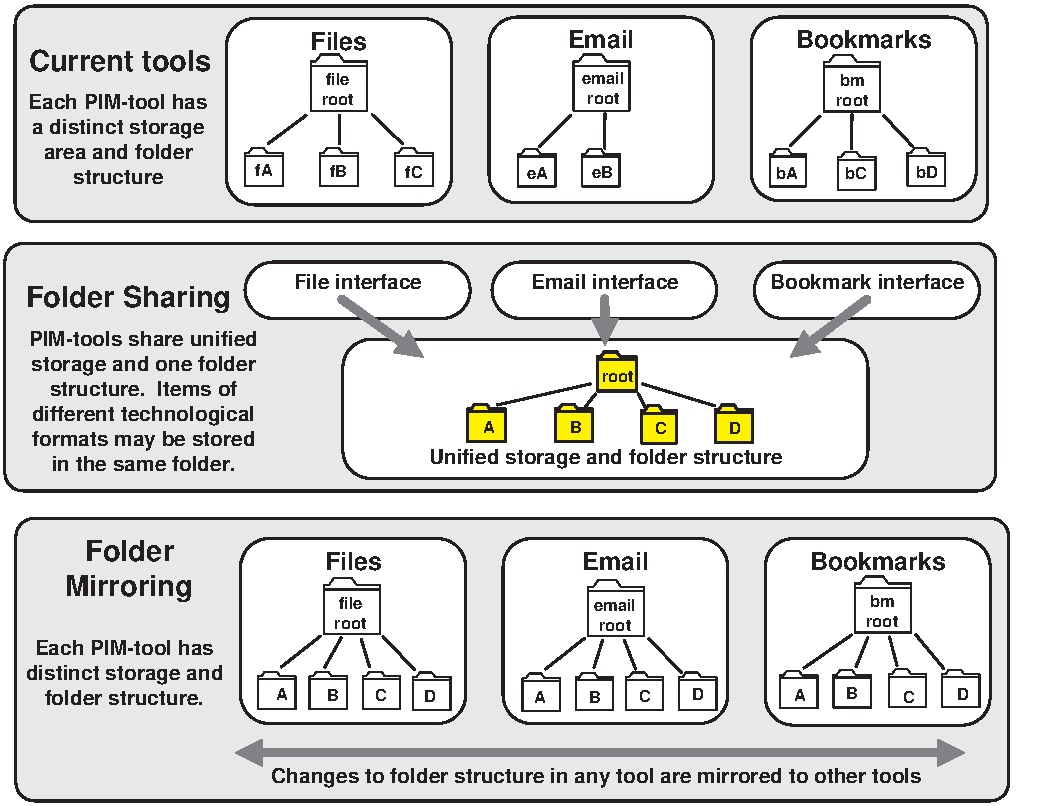
\includegraphics[height=9cm]{pictures/design/Design-fs-fm-comparison.pdf}
		% fs-fm-comparison.pdf}
	\end{center}
	\caption{Comparison of folder-sharing and folder-mirroring}
	\label{fig:design:fs-fm-comparison}
\end{figure}






%%%%%%%%%%%%%%%%%%%%%%%%%%%%%%%%%%%%%%%%%%%%%%%%%%%%%%%%%%%%%%%%%%%%%%%%%%%%%%%%%%
%%%%%%%%%%%%%%%%%%%%%%%%%%%%%%%%%%%%%%%%%%%%%%%%%%%%%%%%%%%%%%%%%%%%%%%%%%%%%%%%%%
%%%%%%%%%%%%%%%%%%%%%%%%%%%%%%%%%%%%%%%%%%%%%%%%%%%%%%%%%%%%%%%%%%%%%%%%%%%%%%%%%%
%%%%%%%%%%%%%%%%%%%%%%%%%%%%%%%%%%%%%%%%%%%%%%%%%%%%%%%%%%%%%%%%%%%%%%%%%%%%%%%%%%






%%%%%%%%%%%%%%%%%%%%%%%%%%%%%%%%%%%%%%%%%%%%%%%%%%%%%%%%%%%%%
\newpage
\section{Design Focus: Folder mirroring}
\label{design:sharing-mirroring}
%%%%%%%%%%%%%%%%%%%%%%%%%%%%%%%%%%%%%%%%%%%%%%%%%%%%%%%%%%%%%
% Can I explain in terms of psychological claims, grounded in basic-science theories, common sense argumentation 
%%%%%%%%%%%%%%%%%%%%%%%%%%%%%%%%%%%%%%%%%%%%%%%%%%%%%%%%%%%%%
% Motivation: consider different types of user?
%%%%%%%%%%%%%%%%%%%%%%%%%%%%%%%%%%%%%%%%%%%%%%%%%%%%%%%%%%%%%
This section describes the design focus in the thesis, the principle of \textit{folder-mirroring} -- allowing the user to replicate changes made to the folder structure in one tool to the folder structures in other tools. \textbf{Section~\ref{design:mirroring:evidence}} presents the empirical and methodological design rationale behind this focus.
% \textbf{Section~\ref{design:mirroring:options}} presents the initial design options that were considered.
\textbf{Section~\ref{design:core-functionality}} describes the core functionality of folder-mirroring in terms of changes to the interaction model of the standard folder hierarchy.
% Then \textbf{Section~\ref{design:rationale}} summarises the key methodological rationale behind this design focus. 

%%%%%%%%%%%%%%%%%%%
% KEY DECISION
%%%%%%%%%%%%%%%%%%%
% This decision is considered as a first focus within the initial design space.  Then a specialization of folder sharing, folder mirroring is presented.
% Folder-sharing is contrasted with related prototypes to date.

%%%%%%%%%%%%%%%
% CORE IDEA
% Present as a cross-tool design -- trying to improve cross-tool support for PIM. Theoretical interest.
%%%%%%%%%%%%%%%

%%%%%%%%%%%%%%%%%%%%%%%%%%%%%%%%%%%%%%%%%%%%%%%%%%%%%%%%%%
\subsection{Design Rationale}
\label{design:mirroring:evidence}
%%%%%%%%%%%%%%%%%%%%%%%%%%%%%%%%%%%%%%%%%%%%%%%%%%%%%%%%%%

%%%%%%%%%%%%%%%%%%
% FROM WM REPORT
%%%%%%%%%%%%%%%%%%
%The qualitative analysis of results revealed a wide range of findings related to the management of multiple hierarchies and the generation of user-defined categories (e.g. folder labels). These can be summarised as follows:
%
% The observation that users generate similar organizational categories in the form of folder labels in different tools within their workspace was a significant step in my thesis work. In other words certain folder names carry meaning across different parts of their workspace. In other words, for some users the outcome of ad-hoc parallel management of personal information is a significant amount of category overlap. In fact some users exerted significant effort towards manually synchronizing the hierarchies.
%
% It confirms that high-level user activities often involve the use of multiple tools, and suggests that many users would welcome the ability to share categories between tools.
%
% The development of WorkspaceMirror was driven by these observations and is intended to act as an evaluation platform for the hypothesis that a significant number of users would benefit from the sharing of hierarchical structure between PIM tools, and the resulting simplification of their workspace.

The next two sections present the empirical and methodological rationale behind the design focus.

%%%%%%%%%%%%%%%%%%%%%%%%%%%%%%%%%%%%%%%%%%%%%%
\subsubsection{Empirical Design Rationale}
%%%%%%%%%%%%%%%%%%%%%%%%%%%%%%%%%%%%%%%%%%%%%%

A number of findings from the exploratory study in \textbf{Chapter~\ref{chapter:exploratory_study}} lead the author to consider the potential benefits for users if they were able to share organizational structure between PIM tools.  Key findings offering evidence in favour of this design route are listed as follows:

%%%%%%%%%%%%%%%%%%%%%%%%
% Motivating factors: Empirical evidence
%%%%%%%%%%%%%%%%%%%%%%%
% laying the groundwork
% Empirical evidence that folder-mirroring may be useful is discussed. 
%%%%%%%%%%%%%%%%%%%%%%%%%%%%%%%%%%%%%%%%%%%%
% BUT: must consider ANGELA'S CLIFF!!!
% why WorkspaceMirror? Why the leap towards integrating the hierarchies?}}
%%%%%%%%%%%%%%%%%%%%%%%%%%%%%%%%%%%%%%%%%%%%
% ALSO: relate to aims (see below)
% %%%%%%%%%%%%%%%
% incremental
% pragmatic
% grounded
% simplifying
%%%%%%%%%%%%%%%%%%%%%%%%%%%%%%%%%%%%%%%%%%%
\begin{enumerate}
%%%%%%%%%%%%%%%%%%%%%%%%%%%%%%%%%%%%%%%%%%%%%%%%%%%%%%%%%%%%%
% Objective evidence: folder overlap (defendable basis?)
%%%%%%%%%%%%%%%%%%%%%%%%%%%%%%%%%%%%%%%%%%%%%%%%%%%%%%%%%%%%%
% Self-obs of overlap
%%%%%%%%%%%%%%%%%%%%%%%%%%%%
% The most common similarity was between files and email (seven participants), e.g. \textit{P1: ``Some structure is overlapping between files and email, my main activities like research and lecturing''}.  However, typically they noted that overlap was partial, often relating to primary roles.  Sometimes folders were sometimes tool-specific, e.g. \textit{P13: `` They [the email folders] are fairly close to the file system, but with some differences. For example this folder contains correspondence-based information which does not make sense in the file system''}.  Overall, many users indicated that PIM-tools shared many folders in common.  This was despite that the fact that each set of user-defined categories was developed separately as a result of compartmentalisation. 
%%%%%%%%%%%%%%%%%%%%%%%%%%%%%%%%%%%%%%%%%%%%%%%%%%%%%%%%%%%%%
%�	For those users who chose to manage more than one folder hierarchy (19 out of 21 of the participants), a significant level of overlap was noted in terms of the categories used to label folders (Boardman 2001a, 2001c.) For some users, the overlap between their file and email hierarchies was as high as 36%. 
%�	Overlapping folders tended to be based on roles, projects and interests (2001b.)
%%%%%%%%%%%%%%%%%%%%%%%%%%%%%%%%%%%%%%%%%%%%%%%%%%%%%%%%%%%%%
\item \textit{Observations of existing folder overlap between different PIM-tools} -- Firstly, the observation of substantial \textit{folder overlap} for many participants, indicated that many users who perform filing in multiple PIM-tools, create similar folders in different tool contexts (see \textbf{Section~\ref{exp-study:Results-folder-overlap}}). Furthermore, during the guided tours, eleven participants highlighted similarities between their folder structures in different tools. Folder overlap suggests that certain user activities are cross-tool and involve the organization of multiple types of information. However, with current tools, each type of information must be organized separately.  Such cross-tool activities therefore involve organizing effort that is distributed: (1) across tools, and (2) over time.

%%%%%%%%%%%%%%%%%%%%%%%%%%%%%%%%%%%%%%%%%%%%%%%%%%%%%%%%%%%%%%%%
% User comments: desire for cross-tool organization support
%%%%%%%%%%%%%%%%%%%%%%%%%%%%%%%%%%%%%%%%%%%%%%%%%%%%%%%%%%%%%%%%
% �	All the subjects emphasised the effort involved in managing multiple types of information in parallel. Note that although the study participants were technically experienced, it can be assumed that these overheads are relevant to all types of user.
% such functionality (e.g. the ability to manage files and email together) was not already provided. 
% Comments: Why do I have to manage files/email etc. separately? Empirical evidence. Quotes.
% participants encountered difficulties whilst managing multiple distinct folder hierarchies. 
% \item As well as folder overlap, other findings suggested that many users may benefit from folder-mirroring.  
\item \textit{Users expressing the wish to share folder structures between tools} -- Several participants complained about the effort of managing multiple collections of personal information separately, and expressed annoyance that it was not possible to manage their files and email together in the same set of folders, e.g.  \textit{P25: ``I suppose not as they've got very distinct usages and purposes but to me it would be easy if I could have everything in one location. But at the moment I have the sense that things are managed in two quite separate ways''}.  % \textit{Although folder-mirroring does not offer such advanced functionality, it does take steps towards this level of integration.}

%%%%%%%%%%%%%%%%%%%%%%%%%%%%%%%%%%%%%%%%%%%%%%%
% Observations of behaviour: manual mirroring
%%%%%%%%%%%%%%%%%%%%%%%%%%%%%%%%%%%%%%%%%%%%%%%
\item \textit{Manual mirroring behaviour} -- Some participants had attempted to manually mirror folders between tools.  These participants reported that it was hard to keep folder structures synchronized, and they tended to diverge over time, \textit{P13: ``All of them [my folder structures] started off with an identical folder structure, but over time they've diverged somewhat''}.  Therefore most had abandoned manual folder-mirroring because of the amount of effort involved, e.g. \textit{P11: ``I maintained my usability knowledge base for 6 months but it was too much hassle and I got out of practice. I want to get restarted in email, file system and web''}.
% They also stated that they tried to keep them in sync, or that they started off in sync, but that it was too much hassle to do manually over time. 
%One participant saved multiple types of information within one folder structure.  She saved email messages as word documents within her file system rather than have to manage another set of folders.
These observations suggested that some users may welcome folder-mirroring. 

%%%%%%%%%%%%%%%%%%%%%%
% Easier retrieval
%%%%%%%%%%%%%%%%%%%%%%
% It was envisaged that consistent organization may also help the user retrieve more effectively.
\item \textit{Difficulties in retrieving information} -- Some participants mentioned problems when retrieving information caused by them not being sure if it was stored in the file collection or the email collection. In particular, retrieval problems were caused by the ability to manage files as attachments within the email collection, e.g. \textit{P22: ``If it wasn't there [in the file folder] I would think damn I forgot to file it in the folder where it belongs and go straight to email''}.  Retrieval problems may be exacerbated by the existence of different organizational structures in each tool. This means that as well as looking in two tools, users may have to look in different locations in each tool. 
% POSSIBLE EXAMPLES files in X, email in Y

\end{enumerate}

%%%%%%%%%%%%%%%%%%%%
% FROM WM REPORT
%%%%%%%%%%%%%%%%%%%%
% The observation that users generate similar organizational categories in the form of folder labels in different tools within their workspace was a significant step in my thesis work. In other words certain folder names carry meaning across different parts of their workspace. In other words, for some users the outcome of ad-hoc parallel management of personal information is a significant amount of folder overlap. 
%
% It confirms that high-level user activities often involve the use of multiple tools, and suggests that many users would welcome the ability to share categories between tools.
%
% The development of WorkspaceMirror was driven by these observations and is intended to act as an evaluation platform for the hypothesis that a significant number of users would benefit from the sharing of hierarchical structure between PIM tools, and the resulting simplification of their workspace.

%%%%%%%%%%%%%%%%%%%%%%%%%%%%%%%%%%%%%%%
% Also consider CONTRASTING counter-arguments
%%%%%%%%%%%%%%%%%%%%%%%%%%%%%%%%%%%%%%%
% Although there was a large amount of evidence in favour of folder-sharing, the author was also aware that there were also counter-arguments.  
The exploratory study also provided evidence that folder-mirroring may \textit{not} be useful.  Folder overlap was in many cases partial, and often limited to certain types of folders such as roles and projects.  In other words, there was some variation in organizational behaviour across the three tools for many participants.
% ADD INTO CHAPTER 4).
Furthermore, some users did not rely on folders and instead relied on sort and search mechanisms.  Therefore would stand to gain little benefit from folder-mirroring.
% Firstly, as noted above, some users stated that they required the flexibility to organize different types of information in different ways -- something which would be inhibited if one set of folders were shared across collections. 

%%%%%%%%%%%%%%%%%%%%%%%%%%%%%%%%%%%%%%%%%%%%%%%%
% Bottom line: interesting area to look at
%%%%%%%%%%%%%%%%%%%%%%%%%%%%%%%%%%%%%%%%%%%%%%%%
%%%%%%%%%%%%%%%%%%%%%%%%%%%%%%
% Empirical investigation
% Interest: do (which?) users do not need different classification schemes for different types of information.
% A key trade-off is identified between PIM overheads and flexibility. % Can this trade-off be expressed in terms of psychological claims along the lines of Carroll? A key sub-issue is identified: how does this trade-off vary between users? 
% Possible Design trade-offs, e.g. overheads versus flexibility. Types of flexibility.
% Real aim: design as test-bed/straw-man -- to explore potential to unify/integrate.
% Explore trade-off's inherent in design (REF: Carroll)
%%%%%%%%%%%%%%%%%%%%%%%%%%%%%%
% Test case/test-bed for/develop methodology, research vehicle to investigate potential to improve integration
% how would users receive the ability to share organizational structure between tools? 
The two sides of this argument indicated that this was be an interesting area to investigate further.  
An implementation of folder-mirroring was envisaged as a research vehicle to investigate the potential of increased integration. The following issues were identified for exploration: how would users respond to the ability to share folders between tools?  Do folder labels carry meaning beyond the boundaries of particular tools?  Do users really need the flexibility to develop distinct classification schemes for different types of personal information? 

%%%%%%%%%%%%%%%%%%%%%%%%%%
% Design hypothesis
%%%%%%%%%%%%%%%%%%%%%%%%%%
% some kind of automatic mechanism could help fulfil this need.  Intuitive need (users need it?), not done manually (too much hassle).  Add similarity of strategies.
The subsequent implementation and evaluation of a folder-mirroring prototype was directed at investigating whether the folder-mirroring mechanism would help users manage the multiple types of information relating to certain activities more effectively.
%%%%%%%%%%%%%%%%%%%%%%%%%
% Speculation: predicted behaviour: Converge over time

%%%%%%%%%%%%%%%%%%%%%%%%%
%%%%%%%%%%%%%%%%%%%%%%%%%%%%%%%%%%%%%%%%%%%%%%%%%%%%%%
% CURRENT: different PIM-tools, manage separately
%%%%%%%%%%%%%%%%%%%%%%%%%%%%%%%%%%%%%%%%%%%%%%%%%%%%%%
% a user can make adjustments to the folder structures in different PIM-tools as required.
In the personal information environment offered by current desktop computers, users must make adjustments separately to the folder structures in different PIM-tools.  Since the folder structures are managed separately, even if users try to keep them synchronized, they tend to diverge over time.  % THINK: would they do this anyway?
With folder-mirroring, it was envisaged that the folder-structures in different collections of personal information may converge.


%%%%%%%%%%%%%%%%%%%%%%%%%%%%%%%%%%%%%%%%%%%%%%%%%%%%%%%%%%
% PERSONAL: Most promising of the prototypes?
% Based on initial feedback from prospective users?
%%%%%%%%%%%%%%%%%%%%%%%%%%%%%%%%%%%%%%%%%%%%%%%%%%%%%%%%%%
% \item As well as relating to an interesting area to study, the author considered this the most promising of the potential designs outlined in \textbf{Section~\ref{design:initial-forays}}.



%%%%%%%%%%%%%%%%%%%%%%%%%%%%%%%%%%%%%%%%%%%%%%%%%%%%%%%%%%
% \subsection{Design rationale}
% \label{design:rationale}
%%%%%%%%%%%%%%%%%%%%%%%%%%%%%%%%%%%%%%%%%%%%%%%%%%%%%%%%%%
% Discuss benefits OVER and BEYOND folder-sharing
% Folder-mirroring retains many of potential benefits of folder-sharing whilst also providing flexibility.
%%%%%%%%%%%%%%%%%%%%%%%%%%%%%%%%%%%%%%%%%%%%%%%%%%%%%%%%%%




%%%%%%%%%%%%%%%%%%%%%%%%%%%%%%%%%%%%%%%%%%%%%%
\subsubsection{Methodological Design Rationale}
%%%%%%%%%%%%%%%%%%%%%%%%%%%%%%%%%%%%%%%%%%%%%%

%%%%%%%%%%%%%%%%%%%%%%%%%%%%%%%%%%%%%%%%%%%%%%%%%%%%%%%%%%
% KEY DESIGN AIM: Incremental
% facilitate up-take of system and effective evaluation
%%%%%%%%%%%%%%%%%%%%%%%%%%%%%%%%%%%%%%%%%%%%%%%%%%%%%%%%%%
% In this section the methodological rationale for this design focus are discussed.
% The focus on folder-mirroring was made for the following reasons:
% Folder-mirroring offers an incremental change relative to current systems. Therefore the design route offers the potential benefits of evolutionary ``hill-climbing'' outlined in \textbf{Section~\ref{design:aims}}.
Folder-mirroring was also seen to be highly compatible with an evolutionary, incremental design route:

\begin{enumerate}

%%%%%%%%%%%%%%%%%%%%%%%%%%%%%%%%%%%%%%%%%%%%%%%%%%%%%%%%%%
% Incremental consequence 2: Few usage barriers
%%%%%%%%%%%%%%%%%%%%%%%%%%%%%%%%%%%%%%%%%%%%%%%%%%%%%%%%%%
\item It was envisaged that folder-mirroring functionality could be applied to existing folder structures, which would be extended incrementally with mirrored folders.  Therefore there are few barriers to initial usage since the user does not have to adjust existing collections in any way. Furthermore, folder-mirroring could be made optional, allowing users to retain the flexibility to organize different types of information in different ways. % i.e.take step towards unification but flexibility is retained.

%%%%%%%%%%%%%%%%%%%%%%%%%%%%%%%%%%%%%%%%%%%%%%%%%%%%%%%%%%
% Incremental consequence 1: Practical/pragmatic route
%%%%%%%%%%%%%%%%%%%%%%%%%%%%%%%%%%%%%%%%%%%%%%%%%%%%%%%%%%
% Step towards PIM-unification in more ambitious schemes - therefore achievable?
% , external constraints -- therefore choice of incremental step, \textit{do-able
%  potential to complete the cycle}
%%%%%%%%%%%%%%%%%%%%%%%%%%%%%%%%%%%%%%
\item Folder-mirroring can be considered a step towards the PIM-integration offered in systems such as MS-WinFS~\citep{winfs:03}.  It was envisaged that this design route represented a practical/pragmatic choice, achievable within the limited time and manpower constraints available, that would provide insight for the developers of more advanced PIM-integration technology.  Based on the author's previous technical experience, it was estimated that the folder-mirroring principle would be possible to implement in a robust way with the limited available time and manpower resources.

%%%%%%%%%%%%%%%%%%%%%%%%%%%%%%%%%%%%%%%%%%%%%%%%%%%%%%%%%%
% KEY DESIGN AIM: EXTENSIBLE
% Lays foundation for more powerful functionality
%%%%%%%%%%%%%%%%%%%%%%%%%%%%%%%%%%%%%%%%%%%%%%%%%%%%%%%%%%
% Longer-term design argument: facilitate project management/knowledge transfer functions
% Folder-mirroring is extendible - it can be built on to provide further PIM integration.
\item Sharing one set of folders across PIM-tools would act as a foundation for more powerful PIM functionality. For example, organizational consistency in this way facilitates the straightforward grouping of related information in different technological formats. Envisaged uses for such cross-tool grouping include collating information for knowledge transfer, starting a new project, or project archiving.
% (``Bill needs to pass on project X to Jane'')
% (``Bill wants to start a new project and wants to create a folder in all his PIM-tools associated with that project'')
% (``Bill is finishing Project X, and wants to archive all related information'')
% A number of design suggestions were received from users in the evaluations reported in \textbf{Section~\ref{design:feasibility-study}} and \textbf{Chapter~\ref{chapter:main-study}}. However in the bulk of the thesis, only the core folder-mirroring functionality is considered.
% Example design steps are outlined (discussed in \textbf{Section~\ref{design:design-extensions}} below, and also under further work in \textbf{Chapter~\ref{chapter:conclusion}}). 

\end{enumerate}









%%%%%%%%%%%%%%%%%%%%%%%%%%%%%%%%%%
\subsection{Core Functionality}
\label{design:core-functionality}
%%%%%%%%%%%%%%%%%%%%%%%%%%%%%%%%%%

%%%%%%%%%%%%%%%%%%%%
% FROM WM REPORT
%%%%%%%%%%%%%%%%%%%%
% The software synchronizes three folder hierarchies: the user's "home directory" where personal documents are stored; (2) web bookmarks stored in the "Favorites" folder; and (3) email messages stored in Microsoft Outlook. WE expect that the software will reduce management overheads, and improve integration for many users - although at the expense of the flexibility to organize different types of information in different ways.

%%%%%%%%%%%%%%%%%%%%%%
% DESCRIBE DESIGN
%%%%%%%%%%%%%%%%%%%%%%
% Discuss as reducing organizational redundancy. Attempt to leverage investment that user is willing to make in structuring their workspace beyond particular tools (promotion of consistency, coherency, positive constraint on user).
% Leverage investment -- support of satisficing. Help users stay organized with less effort (if they want to) and manage the different types of information that they collect in various tools around their workspace. Promote consistency/coherency
%%%%%%%%%%%%%%%%%%%%%%%%%%%%%%%%%%%%%%%%%%%%%%%%%%%%%%%%%%%%%%%%%%%%%%
%	system model to (formally?) describe system}
%	Scenarios are presented to illustrate example situations in which folder-sharing could be used (i.e. confirm the concern/requirement/user need that is the object of design). 
%%%%%%%%%%%%%%%%%%%%%%%%%%%%%%%%%%%%%%%%%%%%%%%%%%%%%%%%%%%%%%%%%%%%%%
% Interface dialogue-level description -- user interaction model
%		\item Relate to the different aspects of PIM
%		\item Scenarios, screen-shots and storyboards
%		\item NB: Not trying to deal with inherent limitations of the hierarchy
%%%%%%%%%%%%%%%%%%%%%%%%%%%%%%%%%%%%%%%%%%%%%%%%%%%%%%%%%%%%%%%%%%%%%%
In this section, the folder-mirroring design is outlined in detail. Firstly,the interactions afforded by the  traditional folder hierarchy are described in terms of three fundamental operations:
%%%%%%%%%%%%%%%%%%%%%%%%%%%%%%%%%%%%%%%%%%%%%%%%
% Functionality of existing folder structures
%%%%%%%%%%%%%%%%%%%%%%%%%%%%%%%%%%%%%%%%%%%%%%%%
% Add a folder
% Delete a folder
% Rename a folder
% THINK: move to folder mirroring?
% The traditional folder hierarchy allows 
\begin{enumerate}
\item \textit{Creating a new folder} -- The folder's location within the folder structure, is defined by the folder's path relative to the root folder. % (e.g. creating folder \texttt{Marylebone} at location \texttt{Root/Train-stations}.
\item \textit{Deleting a folder} -- Items and sub-folders contained within the folder are also deleted.
\item \textit{Renaming a folder} -- In the simplest case, a folder's name is changed, but the folder remains at the same location.  \textit{Moving} a folder can be considered a special case of renaming where the folder's path is changed but the name remains the same.
\end{enumerate}



%%%%%%%%%%%%%%%%%%%%%%%%%%%
% Desired CORE functionality
% Outline interaction model and options thereof. 
% When the user does X, WM offers Y. Scenarios through the functionality.
% Retain 3 different folder structures, but mirror changes between them
% Improve reference to diagram
%%%%%%%%%%%%%%%%%%%%%%%%%%%
The folder-mirroring principle allows the user to replicate the three above operations across multiple folder structures as shown in \textbf{Figure~\ref{fig:design:mirroring}}.  In other words, if a change is made made to the folder structure in one collection, it is replicated to the folder structures in the other collections. % supported by the mechanism.

The core functionality of folder-mirroring, can be defined as follows, in terms of the three above operations: % NB: this is automatic mirroring
\begin{enumerate}

\item \textit{Mirroring the creation of a folder} -- If the user adds a new folder ``C'' in one collection, an equivalent folder ``C'' should be created in the same location in the other collections.  If a folder with that name already exists in that location in one of the other collections, no action should be taken there.

It may be necessary to mirror an entire set of parent folders as follows. Consider the scenario of a folder being mirrored from the file system to email. The file folder in question is \texttt{File-root/A/B}. In email, the intermediate folder, \texttt{Email-root/A} does not exist.  Therefore, the parent folder, \texttt{Email-root/A} must be created before \texttt{B} is created.

\item \textit{Mirroring the deletion of a folder} -- When the user deletes a folder ``C'' in one collection, the equivalent folder (if one exists) should be deleted in the other collections.  If that folder does not exist in one of the other collections, no action should be taken there.

\item \textit{Mirroring the renaming of a folder} -- A scenario is considered when the user renames a folder ``B'' (termed the \textit{source folder}) as folder ``C'' (termed the \textit{destination folder}).  If the source folder exists in one of the other collections at that same location, \textit{and} if the destination folder does not exist, then renaming should be mirrored.  If the source folder does not exist, or the destination already exists in a particular collection, then no action should be taken there\footnote{An alternate design was also considered for renaming, in the case when the source \textit{and} destination folders do not exist in another PIM-tool.  Instead of the action detailed above, the destination folder could be created in the other PIM-tool, and so make the folder structures more consistent.  This alternate design was not implemented in the course of the thesis but remains a possibility for future work.}.
\end{enumerate}

% Examples of the three mirroring operations are shown in \textbf{Figure~\ref{fig:design:mirroring}}.
% %%%%%%%%%%%%%%%%%%%%%%%%%%%%%
% FIGURE - Principles of Mirroring
% %%%%%%%%%%%%%%%%%%%%%%%%%%%%%
%%%%%%%%%%%%%%%%%%%%%%%%%%%%%%%
\begin{figure}[htb]
	\begin{center}
		\leavevmode
		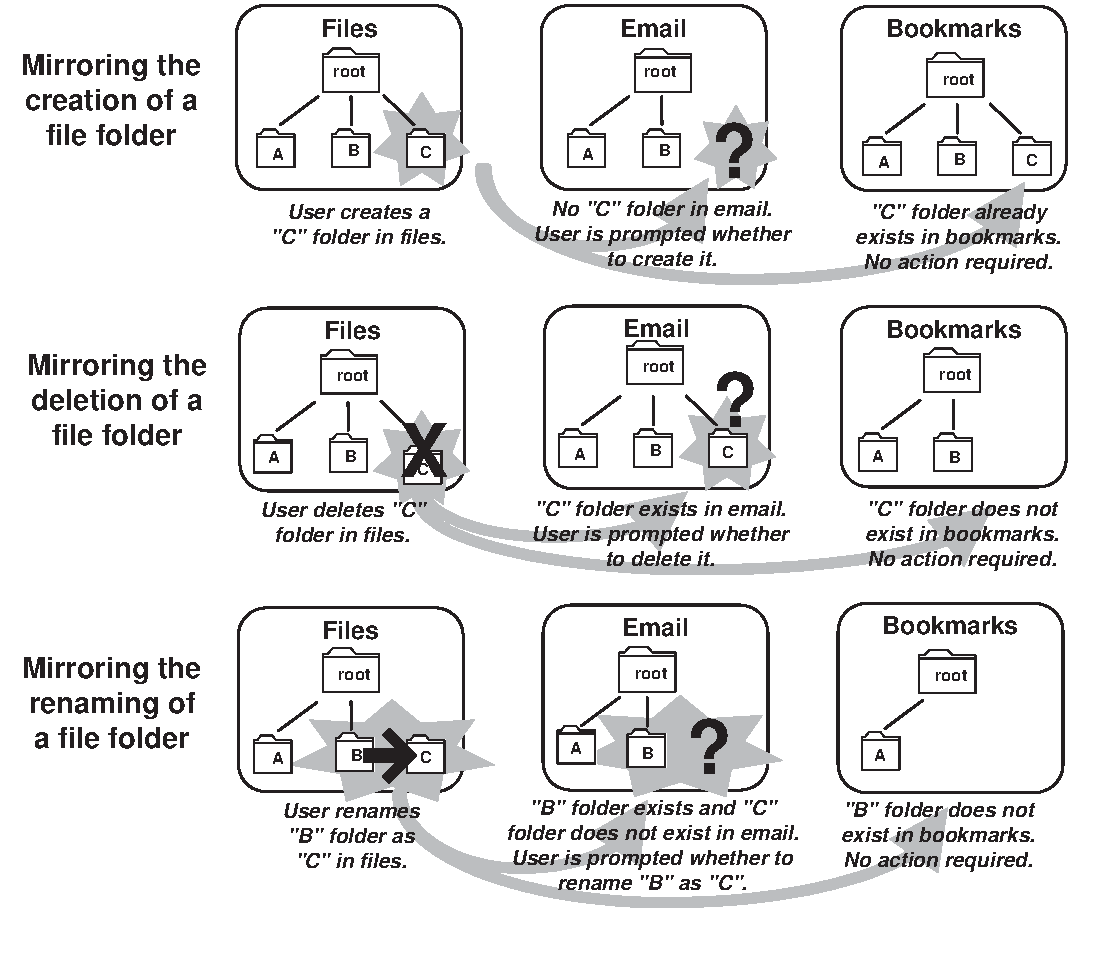
\includegraphics[width=.9 \textwidth]{pictures/design/Design-mirroring.pdf}
	\end{center}
	\caption{Principles of mirroring}
	\label{fig:design:mirroring}
\end{figure}


%%%%%%%%%%%%%%%%%%
% Suitable tools
%%%%%%%%%%%%%%%%%%
The file, email and bookmark collections were deemed suitable for folder-mirroring since they all employ hierarchy-based organizations to arrange items.  Other PIM-tools such as the calendar and contact manager are not suitable because in most cases they do not rely on hierarchical organization\footnote{One can envisage the sharing of folder labels between hierarchy-based tools such as email, and non-hierarchy-based tools such as calendars.  However, this functionality was beyond the scope of the work in this thesis.}.
%%%%%%%%%%%%%
% 2 modes
%%%%%%%%%%%%%
Two modes of operation were envisaged: \textit{automatic} and \textit{manual}. In the automatic mode, folder actions are mirrored automatically. In the manual mode, the user is prompted with a dialogue box as to whether mirroring should be performed.

%%%%%%%%%%%%%%%%%%
% Discussion: NOT ABOUT AN ALTERNATIVE TO THE FOLDER
% Assumption: keep folders.
%%%%%%%%%%%%%%%%%%
% The specific problem being investigated is the current fragmentation between different tools. 
Note that folder-mirroring should not be considered as an attempt to develop an alternative to hierarchical organization.   Limitations of the hierarchy such as single-inheritance~\citep{dourish:99a} are beyond the scope of the thesis.
% The fact is outlined that folder-mirroring is not targeted at providing alternative to the hierarchy.
% Encourage good habits? (risky)
%%%%%%%%%%%%%%%%%%%%%%%%%%%%%%%%%%%%%%%%%%%%%%%%%%%%%%%%%%%%%%%%%%%%%%%%%
% Also, not concerned with providing alternative interaction techniques
%%%%%%%%%%%%%%%%%%%%%%%%%%%%%%%%%%%%%%%%%%%%%%%%%%%%%%%%%%%%%%%%%%%%%%%%%
Also, it should also be noted that folder-mirroring does not provide an alternative means for interacting with folder structures. The user interacts with the three PIM-tools as before (e.g. via direct manipulation, or the command-line).

%%%%%%%%%%%%%%%%%%%%%%%%%%%%%%%%%
\subsubsection{Usage Scenarios}
\label{design:mirroring:scenarios}
%%%%%%%%%%%%%%%%%%%%%%%%%%%%%%%%%

%%%%%%%%%%%%%%
% Scenarios
%  (i.e. confirm the concern/requirement/user need that is the object of design):
%%%%%%%%%%%%%%
Two scenarios were developed, based on comments from the exploratory study, to illustrate how folder-mirroring could be used:
\begin{itemize}

%%%%%%%%%%%%%%%%%%%%%%%
% Creation example
%%%%%%%%%%%%%%%%%%%%%%%
\item \textit{Starting a project} -- Bill is about to embark on a new coding project.  The project involves creating source code and documentation, coordinating with colleagues, and researching information on the internet.  Therefore he predicts that the project will involve the management of associated files, email and bookmarks.
%\begin{enumerate}
%	\item \textit{Create file folder} -- Bill selects his file management tool, navigates to the desired location in the file system, creates the folder, and names it
%	\item \textit{ Create email folder} -- repeat actions as for file folder
%	\item \textit{Create web bookmark folder} -- repeat actions as for file folder
%\end{enumerate}

% Note that in many cases, these actions would not happen sequentially.  PIM is interleaved with the other activities involved in Bill's work, many of which take precedence over PIM.  In fact most users do not have time to manually organize multiple hierarchies, even if they want to. Note also that the sets of actions, if they happen, could happen in any order. Note also that each folder may be located in a different location in the relevant hierarchy.
Using current tools, Bill must create folders separately in each tool in turn.  However, with folder-mirroring, Bill can create a project folder in one location and is then immediately prompted as to whether he wants the folder also created in the other locations. He decides to mirror and the folder is created in the three tool contexts.

%%%%%%%%%%%%%%%%%%%%%%
% Deletion example
%%%%%%%%%%%%%%%%%%%%%%
% Jenny finishes working on "Project Y", after six months working on it flat-out and it being a bane on her life, she doesn't want anything else to do with it. And as one small step towards that she would like it to delete it from her workspace.
% Currently - yet again, three separate sets of actions must be carried out:
%1.	Delete folder in document context
%a.	execute corresponding sub-activities ...
%2.	Delete folder in email context
%a.	execute corresponding sub-activities ...
%3.	Delete folder in web bookmark context.
%a.	execute corresponding sub-activities ...
%
%With WorkspaceMirror Mary would navigate to any PIM tool and delete the folder, after which it would be automatically deleted in the other tools:
%a)	Select a PIM tool (unless user is already there)
%b)	Navigate to desired location in folder hierarchy
%c)	Select "Project Y" and delete it  
%d)	A dialog window appears, asking the user if they also want to delete the folder in the other PIM contexts .
%e)	Transparently the equivalent folders are deleted in the other PIM tools, making use of Recycle Bin facilities where appropriate.
\item \textit{Finishing a project} --  Gemma has just completed a term report on the mating habits of hamsters.  Whilst carrying out this activity, she has managed a large amount of associated files, email and bookmarks within a \texttt{hamster} folder in the respective PIM-tools.  Having backed up the term report itself, Gemma wants to delete all the information relating to the report which are cluttering up her workspace.

Using current tools, she must go to each tool in turn and delete the respective folders and the items they contain.  With folder-mirroring, she is prompted to delete the folder in all three tools, thus saving mouse-clicks and time.  The scenarios assumes that she had previously created the folder in each tool\footnote{Note that an equivalent cross-tool archiving function can also be imagined as an alternative to the cross-tool deletion portrayed in this scenario.}.


%%%%%%%%%%%%%%%%%%%%%
% renaming example
%%%%%%%%%%%%%%%%%%%%%
%Currently Mary also manages each type of personal information separately in distinct tools. Any reorganization must be done performed manually in each tool. Mary currently organizes her work based on project: "Project A", "Project B", "Project C" and so on. Each project is represented by a top-level folder in each of her PIM tools. However on realizing that "Project Z" and "Project A" are both related to one customer "FGH Ltd.", she decides to make this explicit in her workspace. " FGH Ltd." is also represented by a top-level folder in each PIM tool.
%
%Mary must perform three separate sets of actions in three separate tools:
%1.	Move Document folders
%a.	Select document management tool (unless user is already there)
%b.	Navigate to top level in document hierarchy (the file system)
%c.	Select "Project A" and move it into "FGH Ltd.".  
%d.	Repeat for "Project Z"
%2.	Move Email folders
%a.	Select email management tool
%b.	Navigate to top level in email folder hierarchy
%c.	Select "Project A" and move it into "FGH Ltd.".  
%d.	Repeat for "Project Z"
%3.	Move Web Bookmark folders
%a.	Select web bookmark management tool
%b.	Navigate to top level in web bookmark hierarchy
%c.	Select "Project A" and move it into "FGH Ltd.".  
%d.	Repeat for "Project Z"
%
%As before, the interleaved, ad-hoc nature of PIM means that these actions could happen in any order, and few users could be bothered to be so organized.
%
%With WorkspaceMirror Mary would navigate to any PIM tool and carry out her reorganization, after which it would be mirrored in the other tools:
%1.	Move folders in any PIM context
%a)	Select a PIM tool (unless user is already there)
%b)	Navigate to desired location in folder hierarchy
%c)	Select "Project A" and move it into "FGH Ltd.".  
%d)	A dialog window appears, asking the user if they also want to move the folder in the other PIM contexts .
%e)	Transparently the equivalent folders are moved in the other PIM tools.
%f)	Repeat for "Project Z"

\end{itemize}


%%%%%%%%%%%%%%%%%%%%%%%%%%%%%%%%%%%%%%%%%%%%%%%%%%%%%%%%%%%%%%%%%%%%%%%%%%%%%%%%%%
%%%%%%%%%%%%%%%%%%%%%%%%%%%%%%%%%%%%%%%%%%%%%%%%%%%%%%%%%%%%%%%%%%%%%%%%%%%%%%%%%%
%%%%%%%%%%%%%%%%%%%%%%%%%%%%%%%%%%%%%%%%%%%%%%%%%%%%%%%%%%%%%%%%%%%%%%%%%%%%%%%%%%
%%%%%%%%%%%%%%%%%%%%%%%%%%%%%%%%%%%%%%%%%%%%%%%%%%%%%%%%%%%%%%%%%%%%%%%%%%%%%%%%%%




%%%%%%%%%%%%%%%%%%%%%%%%%%%%%%%%%%%%%%%%%%%%%%%%%%%%%%%%%%
%%%%%%%%%%%%%%%%%%%%%%%%%%%%%%%%%%%%%%%%%%%%%%%%%%%%%%%%%%
\newpage
\section{Prototype Implementation}
\label{design:wm-prototyping}
%%%%%%%%%%%%%%%%%%%%%%%%%%%%%%%%%%%%%%%%%%%%%%%%%%%%%%%%%%
%%%%%%%%%%%%%%%%%%%%%%%%%%%%%%%%%%%%%%%%%%%%%%%%%%%%%%%%%%
% WorkspaceMirror: a PIM-unification prototype % based on folder mirroring}
% Add to discussion:

%%%%%%%%%%%%%%%%%%%%%%%%%%%%%%%%%%%%%%%%%%%%%%%%%%
%Design constraints (from core functionality):
%%%%%%%%%%%%%%%%%%%%%%%%%%%%%%%%%%%%%%%%%%%%%%%%%%
%	\item Initial design constraints: desktop workspace
%	\item The decision was taken to mirror folders between three tools - the file system, email and web bookmarks.
%	\item Extension of standard tools -- for familiarity

%%%%%%%%%%%%%%%%%%%%%%%%%%%
% Introduce section
%%%%%%%%%%%%%%%%%%%%%%%%%%%
% Firm belief in firmware.
% Therefore next step was to prototype the design in order to explore pros versus cons.
% Focus on subset of core issues
% Key aims: robustness and long-term usability
This section describes the implementation of a folder-mirroring prototype, \textit{WorkspaceMirror} (abbreviated in this thesis as WM).
%%%%%%%%%%%%%%%%%%%%%%%%
% Choice of platform
%%%%%%%%%%%%%%%%%%%%%%%%
Development was carried out on the MS-Windows desktop operating system, using the languages MS-Visual Basic 6.0 and MS-Visual Basic.NET.  The popular MS-Windows operating system was selected so as to provide access to the largest possible number of potential users.  %Visual Basic was selected due to its status as a development tool suitable for rapid interface prototyping.  % add ~\citep{}.
% See below for reasons for 2 different versions
Rather than recounting the rounds of iterative development and testing performed by the author, a focus is taken on the final architecture of WM.  % However, key design decisions are detailed.


%%%%%%%%%%%%%%%%%%%%%%%%%%%%%%
% Implementation outline
%%%%%%%%%%%%%%%%%%%%%%%%%%%%%%
% WorkspaceMirror has been implemented under MS Windows and synchronizes changes made to the folder hierarchies in three tools: (1) email folders in MS Outlook, (2) the user's document area in the file system, and (3) bookmark folders stored under Favorites. 
WM runs as a background application, monitoring for the creation, deletion, or renaming of folders in three PIM-tools:
\begin{enumerate}

\item \textit{One user-selected area of the file collection} --  The exploratory study highlighted that users often store personal files in multiple locations such as the desktop, the local hard disk, and drives on remote servers.  It was decided to focus on one area of the file system (e.g. ``My Documents'') for two reasons: (1) to enable straightforward mirroring with the email and bookmark collections which are each centred on one primary folder structure, and (2) to enable fast implementation.

\item \textit{MS-Outlook (email collection)} -- A wide range of email clients are in common usage including MS-Outlook, Eudora, Netscape and MS-Outlook Express.  Initial investigation revealed that each client employs incompatible storage formats meaning that it was not possible to support all the clients within the limited time available.  MS-Outlook was chosen as the supported  client because: (1) it possessed a well-defined API accessible from Visual Basic, and (2) it was the most common client encountered in the exploratory study. % chosen as a common email reader with an API that was easily accessible from Visual Basic

\item \textit{MS-Internet Explorer (bookmark collection, also known as ``Favorites'')} -- MS-Internet Explorer was selected as the most common web browser on the MS-Windows platform.

\end{enumerate}

%%%%%%%%%%%%%%%%%%%%%%%%%%%%%%%%%%
% Runs in background - 2 modes
%%%%%%%%%%%%%%%%%%%%%%%%%%%%%%%%%%
WM operates in one of two modes: \textit{automatic} or \textit{prompted}. A configuration setting allows switching between the two modes. In automatic mode, events are mirrored without user intervention.  In prompted mode, WM runs in the background except for prompting the user when the user performs a folder-related operation.  The creation, deletion or renaming of any folder causes a dialogue box to be displayed asking the user if they want to replicate the operation in the other two tools.  An example dialogue box is shown in \textbf{Figure~\ref{fig:design:wm-dialogue}}.  Each of the three PIM-tools are represented by a check box, which can be selected to request mirroring to be performed in that tool. The check box corresponding to the PIM-tool which has sourced the event is hashed out.  A configuration setting allows the user to specify whether the check boxes are enabled or disabled by default. If the check boxes are enabled by default, simply pressing the 'OK' button on the dialogue box causes mirroring to proceed. 


% \textbf{Figure~\ref{fig:design:wm-dialogue}} shows a sample dialogue.
% %%%%%%%%%%%%%%%%%%%%%%%%%%%%%
% FIGURE - example dialogue
% %%%%%%%%%%%%%%%%%%%%%%%%%%%%%
%%%%%%%%%%%%%%%%%%%%%%%%%%%%%%%
\begin{figure}[htbp]
	\begin{center}
		\leavevmode
		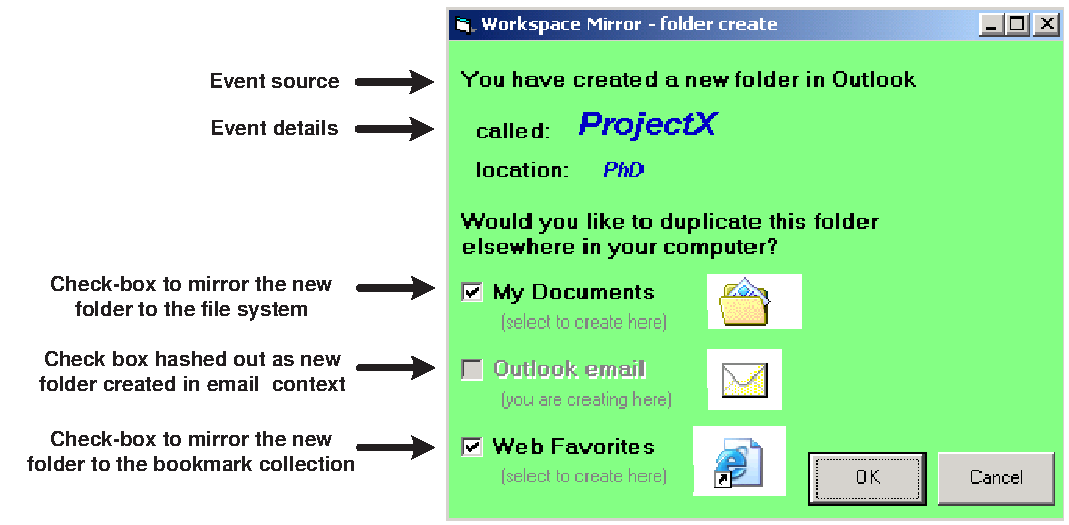
\includegraphics[width=.8 \textwidth]{pictures/design/Design-dialogue.pdf} % Design-dialogue.pdf}
	\end{center}
	\caption{Example WM dialogue: the folder \texttt{PhD/ProjectX} has been created in email.}
	\label{fig:design:wm-dialogue}
\end{figure}

% %%%%%%%%%%%%%%%%%%%%%%%
% Architecture
% %%%%%%%%%%%%%%%%%%%%%%%
\textbf{Figure~\ref{fig:design:architecture}} describes the architecture of the WM prototype, which consists of four main components: (1) \texttt{dotNetWatcher}, (2), \texttt{OutlookWatcher}, (3) \texttt{EventProcessor}, and (4) \texttt{Mirrorer}\footnote{Most of the application coding was performed in MS-Visual Basic 6.0. The only exception was the \texttt{dotNetWatcher} component which was coded in MS-Visual Basic.NET. This version was selected since it offered significantly enhanced support for file system monitoring through the \texttt{FileSystemWatcherClass} class. The \texttt{dotNetWatcher} component communicates with the other components via the ``COM/.Net interop'' mechanism. Since MS-Visual Basic.NET was a beta product at the time of development (Summer/Autumn 2002),  integration between the COM and .NET components was coded manually and was non-trivial.}.  
% \texttt{dotNetWatcher} was implemented in Visual Basic .NET, whilst Visual Basic 6.0 was used for the other three components. 

% The prototype architecture is described in \textbf{Figure~\ref{fig:design:wm-architecture}}.
% %%%%%%%%%%%%%%%%%%%%%%%%%%%%%
% FIGURE - basic architecture and event model
% %%%%%%%%%%%%%%%%%%%%%%%%%%%%%
%%%%%%%%%%%%%%%%%%%%%%%%%%%%%%%
\begin{figure}[htbp]
	\begin{center}
		\leavevmode
		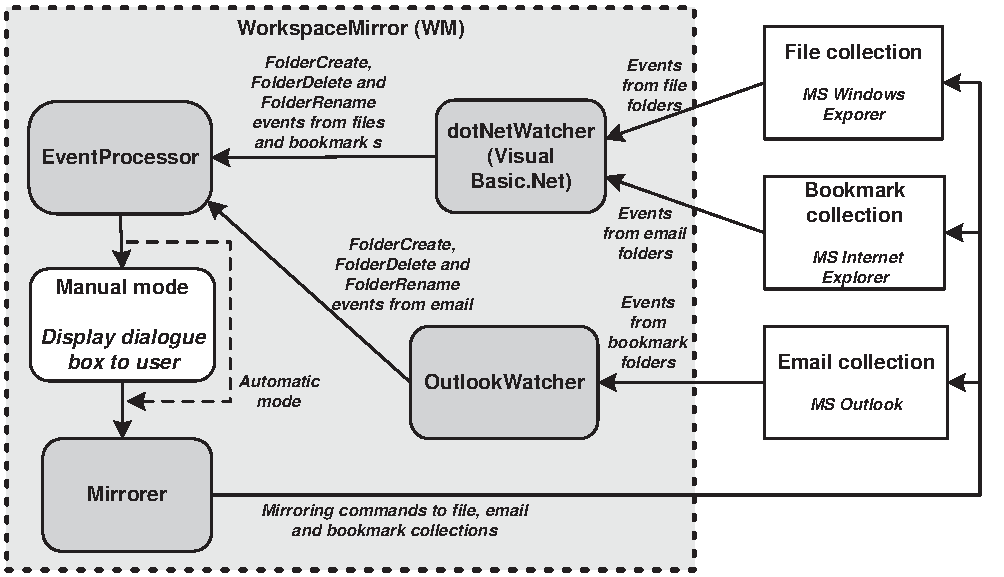
\includegraphics[width=.8 \textwidth]{pictures/design/Design-architecture.pdf}
	\end{center}
	\caption{WorkspaceMirror: overview of technical architecture}
	\label{fig:design:architecture}
\end{figure}

%%%%%%%%%%%%%%%%%%%%%%%%%%%%%%%%%%%%%%%
% dotNetWatcher and OutlookWatcher
%%%%%%%%%%%%%%%%%%%%%%%%%%%%%%%%%%%%%%%
The first two components, \texttt{dotNetWatcher} and \texttt{OutlookWatcher} monitor the three PIM-tools for folder-related events. \texttt{dotNetWatcher} monitors the portions of the file system corresponding to the user's personal files (e.g. ``My Documents''), and bookmarks (termed ``Favorites'' in MS-Windows). \texttt{OutlookWatcher} monitored the folder structure in MS-Outlook. These two components instantiate a \texttt{FolderCreate}, \texttt{FolderDelete} or \texttt{FolderRename} object containing the details of any detected creation, deletion or renaming event. For example the \texttt{FolderCreate} object contains details on the folder name, folder path, and the PIM-tool which generated the event.  All events are then relayed to the 
\texttt{EventProcessor} component.

%%%%%%%%%%%%%%%%%%%%%%
% EventProcessor
%%%%%%%%%%%%%%%%%%%%%%
% Handling recursion
% \item Deletion: avoid cascade of child folder echoes	
The \texttt{EventProcessor} component contains the main application logic for WM. 
Firstly, \texttt{EventProcessor} filters two types of spurious events which are not appropriate for mirroring.
The first type of event are those that relate to default folders (e.g. the creation of a new folder under ``Deleted items'' in email).  \texttt{EventProcessor} maintains a cache of default folders from commonly encountered applications for this purpose.  The \texttt{EventProcessor} component also handles the possibility of event recursion due to folder mirroring.  For example, consider the mirroring of a newly created folder from the file system to email.  The newly mirrored email folder causes a second \texttt{FolderCreate} event to be created, this time by the \texttt{OutlookWatcher} component. \texttt{EventProcessor} avoids event recursion by filtering new events based on a cache of previously mirrored events.   Non-filtered events are processed as follows:
\begin{itemize}

%%%%%%%%%%%%%%%%%%%%%%%%%%%%%%%%%%%%%%%%%%
% Folder creation (name X, location Y)
%%%%%%%%%%%%%%%%%%%%%%%%%%%%%%%%%%%%%%%%%%
\item \textit{FolderCreate event} -- The existence of the folder is checked in the same location in the other PIM-tools.  If there is at least one PIM-tool where there is no corresponding folder, \texttt{EventProcessor} proceeds to mirror the event.  In manual mode, a dialogue box is displayed asking the user if they want to create the folder in those PIM-tools where that folder does not already exist (see \textbf{Figure~\ref{fig:design:wm-dialogue}}).  A configuration setting specifies whether the check boxes are selected by default. Those check-boxes corresponding to the source PIM-tool, and any PIM-tools where the new folder already exists are disabled.  In automatic mode, folders are mirrored automatically as appropriate.
% \item Rebuilding parent chain for creation

%%%%%%%%%%%%%%%%%%%%%%%%%%%%%%%%%%%%%%%%%%%
% Folder deletion: name X, location Y
%%%%%%%%%%%%%%%%%%%%%%%%%%%%%%%%%%%%%%%%%%%
% this is what Cooper might call dangerous functionality.   
\item \textit{FolderDelete event} -- The existence of the folder is verified in the other PIM-tools.  If there is at least one other PIM-tool where the folder exists, \texttt{EventProcessor} proceeds to mirror the event.  In automatic mode, any equivalent folders are deleted automatically\footnote{It may be argued that such ``automatic deletion'' functionality is dangerous as it makes it too easy for the user to remove information without thinking.  Consequently, WM took full advantage of any ``Recycle Bin'' functionality so as to allow the user to restore deleted folders later.}.  In manual mode, a dialogue box is displayed asking the user if they want to mirror the deletion.  As with creation, a configuration setting specifies whether the check boxes are checked by default.  If so, simply clicking OK causes the folder to be deleted in all PIM-tools as appropriate. The check-boxes corresponding to the source PIM-tool, and any PIM-tools where the folder \textit{does not} exist are disabled.


%%%%%%%%%%%%%%%%%%%%%%
% Folder renaming
%%%%%%%%%%%%%%%%%%%%%%
\item \textit{FolderRename event} -- Handling the \texttt{FolderRename} event (from a \textit{source} folder to a \textit{destination} folder) was more complicated.  Mirroring proceeded if in at least one other PIM-tool, the source folder existed and the destination folder did not.  In automatic mode, mirroring proceeds automatically.  In manual mode, a dialogue box is displayed asking the user whether the event should be mirrored to appropriate PIM-tools (i.e. those where the source folder to be renamed exists, and the destination folder does not).  There were implementation difficulties with the handling of \texttt{FolderRename} events. These are discussed in \textbf{Section~\ref{design:implementation-challenges}} below.

\end{itemize}

%%%%%%%%%%%%%%%%%%%
% Final mirroring
%%%%%%%%%%%%%%%%%%%
The \texttt{Mirrorer} component provided the low-level mirroring functionality. Firstly, it repeated the safety checks made by the \texttt{EventProcessor} (e.g. that a folder to be created does not already exist).  \texttt{Mirrorer} also handled various exceptional cases. For example, consider the mirroring of a newly-created \texttt{Email-root/Projects/MondayDemo} folder from email to the file system.  If the parent folder \texttt{File-root/Projects} does not exist in the file system, it must be created before the \texttt{MondayDemo} folder is created.
% Rebuilding parent chain for creation: need to add above?



%%%%%%%%%%%%%%%%%%%%%%%%%%%%%%%%%%%%%%%%%%%%
\subsection{Implementation Challenges}
\label{design:implementation-challenges}
%%%%%%%%%%%%%%%%%%%%%%%%%%%%%%%%%%%%%%%%%%%%

%%%%%%%%%%%%%
% Challenges
% Key challenges which had an impact on user experience are listed below:
%%%%%%%%%%%%%
The development process posed a number of significant technical challenges.  These are briefly surveyed, along with consequent design decisions, as follows:  % described in this section along with consequent design decisions made in the WM prototype that was evaluated in the studies described in \textbf{Section~\ref{design:feasibility-study}} and \textbf{Chapter~\ref{chapter:main-study}}:
\begin{itemize}


%%%%%%%%%%%%%%%%%%%%%%%%%%%%%%%%%%%%%%
% temporary spoof MS-Windows folders
%%%%%%%%%%%%%%%%%%%%%%%%%%%%%%%%%%%%%%
\item MS-Windows creates temporary ``\texttt{New folder}'' and ``\texttt{Copy of X}'' folders when the user creates or copies a file folder.  They must then be renamed by the user as required.  Application logic was added to the \texttt{EventProcessor} module to filter these events to prevent mirroring before they were renamed.  Events corresponding to the renaming of ``\texttt{New Folder}'' or ``\texttt{Copy of X}'' folders are mapped to a \texttt{FolderCreate} event.

%%%%%%%%%%%%%%%%%%%%%%%%%%%%%%%%%%
% Inbox pseudo-root in Outlook
%%%%%%%%%%%%%%%%%%%%%%%%%%%%%%%%%%
% CONSIDER: adding a new DIAGRAM showing email double-root issue
% different hierarchy forms in each tool)
% Outlook but not legal in a folder name in Windows Explorer or Internet Explorer. Casing issues unresolved
\item Differences between the PIM-tools in terms of their folder hierarchy implementation raised a number of challenges.
%%%%%%%%%%%%%%%%%%%%%%%%%%%%%%%%%%%%%%%%%%%%%%
% Where is the root? There can only be 1!
%%%%%%%%%%%%%%%%%%%%%%%%%%%%%%%%%%%%%%%%%%%%%%
First, within MS-Outlook, a user may create folders beneath the default \texttt{Inbox} folder, or at the root ``\texttt{Personal folders}'' level. This is problematic when mirroring to the file and bookmark collections where it does not make sense to have an \texttt{Inbox} folder.  In the WM prototype described here, it was decided to ignore folders beneath the \texttt{Inbox}. % (see \textbf{Figure~\ref{fig:design:inbox-headache}}). 
Second, MS-Outlook allows ``shell'' characters such as  '\&' and '/' to appear legally in folder names. This is not the case in the MS-Windows file system where such characters are not permitted in folder names. For this reason, events relating to folders containing shell characters in their names were removed by the \texttt{EventProcessor} component, and the user notified that mirroring would not be performed. % Consider future version mod

%%%%%%%%%%%%%%%%%%%%%%%%%%%%%%%%%%%%%%%%
% Limitations in Outlook event model
%%%%%%%%%%%%%%%%%%%%%%%%%%%%%%%%%%%%%%%%
% Only get `change' event on rename or delete of folder. Hard to tell between them
\item MS-Outlook provides a COM interface that generates events when folders are created, deleted and changed. However, some major limitations were encountered.  In particular, the \texttt{delete} and \texttt{rename} events do not convey information about which folder has been deleted or changed. Therefore, \texttt{dotNetWatcher} stores a cache of the email folder hierarchy that can be interrogated to provide this information.

However, significant difficulties in handling the mirroring of rename events in MS-Outlook which involved the movement of a folder between different parent folders (e.g. moving folder \texttt{B} from \texttt{Email-root/A/B} to \texttt{Email-root/C/B}).  The limitations in the MS-Outlook object model, combined with the limited development time available, meant that it was not possible to implement this email event in the evaluated version of the WM prototype.  % A planned extension to WM was intended to provide this functionality by maintaining a cache of the email folder structure.
% A single event, FolderChange, is generated corresponding to the parent folder to which a folder is moved to.
% The initial implementation of WM maintained a cache of email folders and their children, but not one of the entire tree -- thus it was not possible to differentiate delete and renaming events in Outlook. WRONG
% corresponding to a folder X, if X is renamed or a child-folder of X is moved elsewhere. 

%%%%%%%%%%%%%%%%%%%%%%%%%%%%%%%%%%
% Mentioned above in main speel
%%%%%%%%%%%%%%%%%%%%%%%%%%%%%%%%%%
% \item Avoiding recursion (and meta-post-cancel recursion)
%%%%%%%%%%%%%%%%%%%%%%%%%%%%%%%%%%%%%%%%%%%%%%%
% Limited to one folder root in each tool
% OK for proof of concept - POSSIBLE REPEAT WITH ABOVE
%%%%%%%%%%%%%%%%%%%%%%%%%%%%%%%%%%%%%%%%%%%%%%%
% Likewise, in MS-Outlook users may store messages under Inbox or under the ro
\item One acknowledged limitation of WM is that it only monitors the folder structure beneath one root folder in each PIM-tool.  However, in the file system, users may distribute their personal files in multiple locations (e.g. ``My Documents'' and the ``Desktop'').  It was envisaged that a facility for multiple roots within one PIM-tool context could be added in later versions. 


%%%%%%%%%%%%%%%%%%%%%%%%%
% Others to mention?
%%%%%%%%%%%%%%%%%%%%%%%%%
% Varying default folders

\end{itemize}


%%%%%%%%%%%%%%%%%%%%%%%%%%%%%%%
% Consider: Link to appendix
%%%%%%%%%%%%%%%%%%%%%%%%%%%%%%%
% More technical detail is provided in an appendix.


%%%%%%%%%%%%%%%%%%%%%%%%%%%%%%%%%%%%%%%%%%%%%%%%%%%%%%%%%%%%%%%%%%%%%%%%%%%%%%%%%%
%%%%%%%%%%%%%%%%%%%%%%%%%%%%%%%%%%%%%%%%%%%%%%%%%%%%%%%%%%%%%%%%%%%%%%%%%%%%%%%%%%
%%%%%%%%%%%%%%%%%%%%%%%%%%%%%%%%%%%%%%%%%%%%%%%%%%%%%%%%%%%%%%%%%%%%%%%%%%%%%%%%%%
%%%%%%%%%%%%%%%%%%%%%%%%%%%%%%%%%%%%%%%%%%%%%%%%%%%%%%%%%%%%%%%%%%%%%%%%%%%%%%%%%%

% An initial pre-implementation exploration of these usage issues is presented in \textbf{Section~\ref{design:feasibility-study}}. 

%%%%%%%%%%%%%%%%%%%%%%%%%%%%%%%%%%%%%%%%%%%%%%%%%%
%%%%%%%%%%%%%%%%%%%%%%%%%%%%%%%%%%%%%%%%%%%%%%%%%%
\newpage
\section{Initial Evaluation} % Feasibility study}
\label{design:feasibility-study}
%%%%%%%%%%%%%%%%%%%%%%%%%%%%%%%%%%%%%%%%%%%%%%%%%%
% \textit{THINK: location of feasibility study (here - or next chapter?)}
% Give users chance to mirror, do they take it?
%%%%%%%%%%%%%%%%%%%%%%%%%%%%%%%%%%%%%%%%%%%%%%%%%%
%%%%%%%%%%%%%%%%%%%
% Link to next section
%%%%%%%%%%%%%%%%%%%
% does WM meet needs better? Does it open up new possibilities? Cue the need for evaluation.
%\textbf{Section~\ref{design:feasibility-study}} moves on to describe the initial evaluation of WM to establish the viability of the folder-mirroring principle.

% This section describes the feasibility study carried out to assess the viability of folder-mirroring.
The aim of this initial evaluation was to assess the workability of the design, and identify bugs before deploying the tool to users over the long-term.  
%%%%%%%%%%%%%%%%%%%%%%%%%%%%%%%%%%%%%%%
%\subsubsection{Open design issues}
%\label{design:mirroring:open-issues}
% Design issues - to be investigated in the first evaluation
%%%%%%%%%%%%%%%%%%%%%%%%%%%%%%%%%%%%%%%
In particular, feedback was sought regarding several unresolved design questions:
\begin{itemize}

%%%%%%%%%%%%%%%%%%%%%%%%%
% Runs in background
%%%%%%%%%%%%%%%%%%%%%%%%%
% Most of the time, the user is not aware of the folder-mirroring functionality which runs in the background, seemingly as part of the operating system.  
\item What feedback should be provided to indicate that WM is running and folder-mirroring is operational?

%%%%%%%%%%%%%%%%%%%%%%%%%
% Modes of operation
%%%%%%%%%%%%%%%%%%%%%%%%%
\item Do users prefer WM to operate in automatic or manual modes?

%%%%%%%%%%%%%%%%%%%%%%%%%
% Mirror by default?
% Possible Design trade-offs, e.g. overheads versus flexibility. Types of flexibility.
%%%%%%%%%%%%%%%%%%%%%%%%%
% consistency of organizational structures across tools
\item Should mirroring be enabled or disabled by default in the dialogue box? % Such a decision impacts the design of the dialogue box (whether the tick boxes for different tools are enabled or not). % Turning mirroring on by default, would improve the ease of mirroring, but potentially impact flexibility.  

\end{itemize}




%%%%%%%%%%%%%%%%%%%%%
\subsection{Method}
%%%%%%%%%%%%%%%%%%%%%

Five colleagues of the author took part in the initial evaluation (see \textbf{Table~\ref{table:design:user_summary}}.)  Three (F1, F2 and F4) had previously taken part in the exploratory study described in \textbf{Chapter~\ref{chapter:exploratory_study}}.  Four (F1, F2, F3, F5) also agreed to subsequently take part in the long-term study described in \textbf{Chapter~\ref{chapter:main-study}}.  Previous to the evaluation described here, all five participants relied on folders for organizing their file, email and bookmark collections. % (ADD CROSS-TOOL PROFILE). 

Participants were interviewed as follows.  Firstly, WM was installed on the participant's main work computer.  The author then introduced WM, and provided a walk-through of folder mirroring.  WM was deployed in prompted mode, so as to give more control over the mirroring process.  Participant were then asked to try out the tool and provide feedback on any aspect of the design.  Data was collected in the form of notes taken by the author.
% add details on time?
 
% During the study, participants were asked whether they preferred the prompted or automatic modes of operation.
% and allow them to retain the flexibility to organize each collection differently.

%%%%%%%%%%%%%%%%%%%%%%%%%%%%%%%%%%%%%%%%%%%%%%%%%%%%%%%
% TABLE: initial evaluation participants
%%%%%%%%%%%%%%%%%%%%%%%%%%%%%%%%%%%%%%%%%%%%%%%%%%%%%%%
\begin{table}[hbtp]
\begin{center}
\begin{footnotesize}
\setlength{\extrarowheight}{2pt}
% Table generated by Excel2LaTeX from sheet 'FEASABILITY EVAL'
\begin{tabular}{|c|p{2.5cm}|p{2.5cm}|c|c|c|c|c|p{2.5cm}|}
\hline
  {\bf ID} & {\bf ID in Exploratory Study (Chapter~\ref{chapter:exploratory_study})} & {\bf ID in Main Study (Chapter~\ref{chapter:main-study})} &  {\bf Age} &  {\bf Sex} & {\bf Job role} & {\bf OS} & {\bf Cross-tool profile} \\
\hline
        F1 &         P1 &        M1 &      35-40 &          M &   Academic & Win2000 & CT2 (F1, E2, B2) \\
\hline
        F2 &         P2 &        M2 &      20-25 &          M &    Student & Win2000 & CT1 (F1, E2, B1) \\
\hline
        F3 &          - &        M3 &      20-25 &          M &    Student & Win2000 & CT3 (F1, E3, B2) \\
\hline
        F4 &        P23 &          - &      30-35 &          M &    Student & WinXP & CT2 (F2, E1, B2) \\
\hline
        F5 &          - &        M4 &      30-35 &          F &    Student & WinXP & CT1 (F2, E2, B1) \\
\hline
\end{tabular}  
\end{footnotesize}
\caption{Participants in initial evaluation of WM}
\label{table:design:user_summary}
\end{center}
\end{table}
\normalsize


%%%%%%%%%%%%%%%%%%%%%%%
\subsection{Results}
%%%%%%%%%%%%%%%%%%%%%%%
% MOVE TO MAIN STUDY: Although there was not always a direct one-to-one mapping between their folder requirements in each tool, they welcomed the chance to reflect on the relevance of the organizational decisions made in one tool, to other contexts.   Occasionally mirrored folders were not always used for the storage of items in all tools, but the testers indicated that the improved consistency outweighed the side effect of increased clutter.  
% The users also reported lower management overheads and easier retrieval of filed items, however WE have not yet attempted to confirm these results objectively.  
% Two users mirrored mostly between the document and email collections, whilst the third mirrored between all three tools. In general mirroring was seen to be most useful for high-level folders, which tended to be based on cross-tool projects and roles.

Four of the participants provided positive feedback. They found the idea of mirroring folders between tools both intuitive and compelling, and welcomed the increased consistency between the three folder structures that they predicted would result from extended use of WM.  For instance, participant F1 stated, \textit{``You only have to create a folder once ...  you create a [file] folder, you create a word document in that folder -- and the next thing you think oh I have to do a web search on the topic.  So you do a web search and you find some interesting websites, but you don't really have to think about where you're going to store those websites''}.  Participant F2 foresaw one situation where he would find folder-mirroring particularly useful: \textit{``One scenario where I would currently use it would be when I'm browsing the web for software ... I always create a new web bookmark and document folder manually with the same names''}.

However, the feedback from these four users was not entirely positive.  Two of the four also observed that there was not always a one-to-one mapping between the folder structures in different PIM-tools. They stated that not all folder operations should be mirrored between tools due to differing organizational requirements, e.g. F1: \textit{``In the web bookmarks, you might have sub-folders which are slightly different than the ones you want in the file system. So in my web bookmarks I might want to say I've got projects called `semantic web' and `XML' ... But you don't really want to do that in the file system because whatever report you're going to write one report about the semantic web and one about XML''}. % , but then you would then have the sub-folders - but they might be different between the two''}. 
% [DF/PROB/MAPPING]  BUT at the top level I think its very useful. Just from my experience, from the way I do things - somebody else may totally disagree. 
% Two participants suggested that mirroring may be most appropriate for top-level folders relating to \textit{``high-level activities such as my thesis, the papers I'm working on, personal stuff, and big projects'' (F2)}.
%%%%%%%%%%%%%%%%%%%%%%%%%%%%%%%%%%%%%%%%%%%%%%%%%%%%%
% Bootstrapping: consider moving to next chapter
%%%%%%%%%%%%%%%%%%%%%%%%%%%%%%%%%%%%%%%%%%%%%%%%%%%%%
Two participants also expressed concern regarding the bootstrapping of the system, i.e. its incorporation within an existing working habits, e.g. F5: \textit{``It's all a matter of getting into the habit.  It's difficult when you start but you get used to it''}. Longer-term evaluation was deemed necessary to explore issues relating to the adoption of the mechanism within a well-developed personal information environment.

The final participant (F3) was much less positive and provided a useful counter-example.  He did not see any point in mirroring folders between the three tools.  He was the most \textit{organizing-neutral} of the five participants.  Although he performed some organizing in files, he filed very few emails or bookmarks.  He also found the idea of prompting intrusive.  % However, towards the end of the interview he indicated that he may find the tool more useful when setting up a new project for the first time. He also suggested that users setting up a computer for the first time may find it useful.
Despite his reservations he agreed to leave the software running to test its robustness.

%%%%%%%%%%%%%%%%%%%%%%
% BUGS IDENTIFIED
%%%%%%%%%%%%%%%%%%%%%%
% Various bugs were identified during the feasibility study.
A number of design recommendations were made by the participants and incorporated in WM before the main evaluation reported in \textbf{Chapter~\ref{chapter:main-study}}:
\begin{itemize}

\item All participants wanted to be made aware that WM was running in the background.  Resulting from this feedback, an animated icon was added to the task bar.

% As noted above, they reported that there was not always a direct one-to-one mapping between their folder requirements in each tool. Therefore they expressed a need to keep close 
\item Participants wanted to have close control over mirroring and so preferred the prompted mode of operation.  Most participants were not concerned about the intrusion of the dialogue, e.g. F1: \textit{``its not that often that you create new folders anyway''}.   However, one suggested the dialogue box should carry a ``do not ask me about mirroring again'' check-box.  Three participants wanted the mirroring check-boxes selected by default. 

\end{itemize}

%%%%%%%%%%%%%%%%%%%%%%%%%%%%
% SUGGESTIONS FOR FEEDBACK
%%%%%%%%%%%%%%%%%%%%%%%%%%%%
Feedback also included a number of suggestions for extensions to the core functionality.  The main evaluation was based on the core functionality as described in this chapter. Longer-term design suggestions are discussed along with those from the main evaluation in \textbf{Section~\ref{main-study:results:themes-design-recs}}.

%%%%%%%%%%%%%%%%%%%%%%%%%%
% Windows .NET limitations
% Mapping of charecters Casing limitations of event model in Windows.Net package.
% Windows.Net does not work with samba-mounted drives
% ADD? Finally, Need keep-alive's for Windows.Net object
%%%%%%%%%%%%%%%%%%%%%%%%%%%
% relating to the \texttt{dotNetWatcher} component were uncovered.
During the interviews, several implementation-related issues were also uncovered:
\begin{itemize}
\item The \texttt{FileSystemWatcher} .NET class  was found to be incompatible with UNIX-based network drives (e.g. those mounted via \texttt{Samba}).  In addition, due to a bug in the ``COM/.NET interop'' mechanism, casing information was lost from all folder and path information.  Fixes for these issues were not implemented before evaluation. % CHECK.

%%%%%%%%%%%%%%%%%%%%%%%%%
% Clunky, hard install
%%%%%%%%%%%%%%%%%%%%%%%%%
\item Installation was found to be a time-consuming and intricate process as a .NET library developed by the author had to be installed.  This learning experience proved invaluable for rolling out WM to more users in the main study.  Also, MS-Visual Basic.NET was incompatible with older versions of MS-Windows, meaning that several prospective trial users were ruled out.
% \textit{F3: dialog should carry a checkbox, "display this dialog for next folder creation"}
\end{itemize}

%%%%%%%%%%%%%%%%%%%%%%%%%
\subsubsection{Summary}
%%%%%%%%%%%%%%%%%%%%%%%%%
%%%%%%%%%%%%%%%%%%%%%%%%%%%%%%%%%%%
% Motivate need for main study.
%%%%%%%%%%%%%%%%%%%%%%%%%%%%%%%%%%%
% Wanted to continue in the longer term! The need for long-term field study indicated.
%%%%%%%%%%%%%%%%%%%%%%%%%
% SUMMARY of Results -- three say ``yes'', one say ``no''.  
%%%%%%%%%%%%%%%%%%%%%%%%%
% Confirmed promising direction for further work. Expand. Problems and fixes to design
% % Evaluation was deemed necessary to investigate this trade-off.
In summary, the initial evaluation indicated the potential benefits of folder-mirroring, but also highlighted the need for investigation of the trade-off between the potential benefits of WM such as improved consistency, and downsides such as interruptions caused by the dialogue boxes.  Overall it was decided that a longitudinal study would be worthwhile.



% \item Since WM runs in the background, participants requested a  icon to indicate its operation.  An .  Right-clicking on the icon provided access to WM's configuration panel.


%%%%%%%%%%%%%%%%%%%%%%%%%%%%%%%%%%%%%%%%%%%%%%
% Differentiate core and design extensions
%%%%%%%%%%%%%%%%%%%%%%%%%%%%%%%%%%%%%%%%%%%%%%
%However, in the context of this thesis, the decision was made to focus on the core functionality: folder-mirroring between the local file, email and bookmark collections as described in \textbf{Section~\ref{design:sharing-mirroring}}.
% The subsequent longitudinal study is described in \textbf{Chapter~\ref{chapter:main-study}}.


%%%%%%%%%%%%%%%%%%%%%%%%%%%%%%%%%%%%%%%%%%%%%%%%%%%%%%%%%%%%%%%%%%%%%%%%%%%%%%%%%%
%%%%%%%%%%%%%%%%%%%%%%%%%%%%%%%%%%%%%%%%%%%%%%%%%%%%%%%%%%%%%%%%%%%%%%%%%%%%%%%%%%
%%%%%%%%%%%%%%%%%%%%%%%%%%%%%%%%%%%%%%%%%%%%%%%%%%%%%%%%%%%%%%%%%%%%%%%%%%%%%%%%%%
%%%%%%%%%%%%%%%%%%%%%%%%%%%%%%%%%%%%%%%%%%%%%%%%%%%%%%%%%%%%%%%%%%%%%%%%%%%%%%%%%%


%%%%%%%%%%%%%%%%%%%%%%%%%%%%%%%%%%%%%%%%%%%%%%%%%%%%%%%%%%%%%%%%%%%%%%%%%
%%%%%%%%%%%%%%%%%%%%%%%%%%%%%%%%%%%%%%%%%%%%%%%%%%%%%%%%%%%%%%%%%%%%%%%%%
\newpage
\section{Discussion}
\label{design:discussion}
%%%%%%%%%%%%%%%%%%%%%%%%%%%%%%%%%%%%%%%%%%%%%%%%%%%%%%%%%%%%%%%%%%%%%%%%%
%%%%%%%%%%%%%%%%%%%%%%%%%%%%%%%%%%%%%%%%%%%%%%%%%%%%%%%%%%%%%%%%%%%%%%%%%

%%%%%%%%%%%%%%%%%%%%%%%%%%%%%%%%%%%%%%%%%%%%%%%%%%%%%
This section compares the WM prototype with other related PIM technology.
%%%%%%%%%%%%%%%%%%%%%%%%%%%%%%%%%%%%%%%%%%%%%%%%%%%%%
% Apple Mail.app - stores attachments in mirrored hierarchy of attachment folders (mirrored on email folders)
%%%%%%%%%%%%%%%%%%%%%%%%%%%%%%%%%%%%%%%%%%%%%%%%%%%%%
% Other research, including our own, is aimed at providing more effective support for PIM-related activities such as task management. 
% Consider the design-space of related PIM unifying systems. (many more ambitious), consider number/type of organizational dimensions
%%%%%%%%%%%%%%%%%%%%%%%%%%%%%%%%%%%%%%%%%%%%%%%%%%%%%
% In this section, folder-mirroring is compared with existing PIM tools and prototypes.
% Re-frame integration from being an ``add-on'' to being ``designed-in'' 
% Implicit (designed-in) integration. 
%%%%%%%%%%%%%%%%%%%%%%%%%%%%%%%%%%%%%%%%%%%%%%%%%%%%%

%%%%%%%%%%%%%%%%%%%%%%%%%
% CURRENT INTEGRATION
%%%%%%%%%%%%%%%%%%%%%%%%%
Firstly, WM can be compared with standard PIM-integration mechanisms.  These are typically aimed at the transfer of information between different tools, e.g. the ``send-to'' facility in MS-Windows.  The author is not aware of any commonly available integration mechanisms that provide the ability to share organizational structure across different PIM-tools.
% WM can also be distinguished from cross-tool search facilities as it is focused on the organization sub-activity.

%%%%%%%%%%%%%%%%%%%%%%%%%
% MS ``My Categories
%%%%%%%%%%%%%%%%%%%%%%%%%
One similar commercial prototype was \textit{``My Categories''}, part of Microsoft's now defunct .NET Services architecture~\citep{myservices:01}. This allowed an individual to store a set of organizational categories on a central server, which could then be imported into different applications.  The system was abandoned by Microsoft over concerns regarding entrusting all personal information to one entity. Furthermore, no evaluations were reported.
% (note that the system also proposed storing email, contacts, tasks and so on).  In addition, no evaluation was published.

%%%%%%%%%%%%%%%%%%%%%%%%%%%%%%%%%%%%%%%
% Similar systems: sharing folders
%%%%%%%%%%%%%%%%%%%%%%%%%%%%%%%%%%%%%%%
Within the research domain, several proposals have been made for the sharing hierarchical folder structure across multiple PIM-tools -- the \textit{subjective classification principle}~\citep{Bergman:03}, and the \textit{Personal Unifying Taxonomy}~\citep{Jones:04}.  Note that both these proposals were published subsequently to the work reported in the thesis.  In addition, unlike WM, neither approach has been prototyped or evaluated.



%%%%%%%%%%%%%%%%%%%%%%%%%%%%%%%%%%%%%%%%%%%%%%
% NOT ALT TO HIERARCHY
%%%%%%%%%%%%%%%%%%%%%%%%%%%%%%%%%%%%%%%%%%%%%%
 % Consider merger with above

%%%%%%%%%%%%%%%%%%%%%%%%%%%%%%%%%%%%%%%%%%%%%%%%%%%%%%%%
% Compare with ambitious PIM-integration prototypes
%%%%%%%%%%%%%%%%%%%%%%%%%%%%%%%%%%%%%%%%%%%%%%%%%%%%%%%%
WM can be considered to be an evolutionary step towards more ambitious research systems that have proposed to unify PIM within a consolidated interface, e.g. \textit{LifeStreams}~\citep{Gelernter:96a}, \textit{Haystack}~\citep{haystack:99}, and \textit{Presto}~\citep{dourish:99a}.
Such revolutionary systems, although exciting in technological terms, were criticised in \textbf{Chapter~\ref{chapter:review}} for a lack of evaluation. In contrast, a prime aim in this work was to facilitate evaluation by pursuing an incremental design based on relatively modest changes to standard software.
This has the added advantage of enabling in situ evaluation with minimal disruption to the users concerned.  These systems also combine multiple design aims, such as developing an alternative to traditional hierarchical organizing mechanisms, as well as unifying the storage of items based in different technological formats. Instead, WM is not concerned with providing an alternative to the folder hierarchy, and it is acknowledged that the limitations of this organizational mechanism are inherited in this incremental design.  WM instead has one design aim -- to allow users to mirror one hierarchical folder structures between different PIM-tools.


%%%%%%%%%%%%%%%%%%%%%%%%%%%%%%%%%%%%%%%%%%%
% Compare with primary org-dim systems
%%%%%%%%%%%%%%%%%%%%%%%%%%%%%%%%%%%%%%%%%%%
Other PIM-integration prototypes have offered users a unified organizational hierarchy based on a particular organizational dimension, e.g. \textit{RoleManager}~\citep{Shneiderman:94} and \textit{UMEA}~\citep{Kaptelinin:03}. In contrast, WM allows the user to develop folders based on arbitrary organizational dimensions.  The results in \textbf{Section~\ref{exp-study:Results-org-dims}} illustrated that this was important for many of the study participants.

%%%%%%%%%%%%%%%%%%%%%%%%%%%%
% Compare with embedding
%%%%%%%%%%%%%%%%%%%%%%%%%%%%
%%%%%%%%%%%%%%%%%%%%%%%%%%%%%%%%%%%%%%%%%%%%%%%%%%%%%%%%%%
% KEY DESIGN AIM: SIMPLIFICATION
%%%%%%%%%%%%%%%%%%%%%%%%%%%%%%%%%%%%%%%%%%%%%%%%%%%%%%%%%%
% Move towards Universal Usability~\citep{Shneiderman:00}}
% Attempt to simplify workspace~\citep{web-good-easy:01}
% Notion of constraints.  Relationship of power/flexibility with overheads/complexity.  Traditional constraints and inverse paradox of power constraints.
%%%%%%%%%%%%%%%%%%%%%%%%%%%%%%%%%%%%%%%%%%%%%%%%%%%%%%%%%%
% Not aim for a particular type of user
% This design work set out to be more universal and aimed for a simple approach to PIM integration.  
% Aimed at range of users (not specifically techies)
% Avoid increase in complexity of individual tools (compare with embedding strategy).
% Take deliberate steps towards reducing complexity? User dislike for advanced features, avoid bloating
%%%%%%%%%%%%%%%%%%%%%%%%%%%%%%%%%%%%%%%%%%%%%%%%%%%%%%%%%%
It is the view of the author that many previous PIM-integration mechanisms have been highly complex, and thus add to the complexity of already complex tools. Indeed most of the design work has implicitly acknowledged this point by aiming prototypes at technically experienced users.  A key concern in this work was to avoid increasing the existing complexity of current interfaces~\citep{mcgrenere:02}, and if possible, to reduce complexity.  The need to simplify PIM-tools has been previously called for by~\citet{web-good-easy:01}.  The design of WM is based on the sharing of PIM functionality \textit{between} PIM-tools, namely the folder structure in which items are organized.  Rather than having to manage different organizational schemes for different types of personal information (e.g. files, email and bookmarks), folder-mirroring makes it possible to share one organizational structure across all. In this way, folder-mirroring can be considered to be a ``simplifying'' PIM design that provides benefits to the user through improved consistency.   This stands in contrast with the recent design trend for \textit{embedding} support for managing non-native types of information such as to-dos within email~\citep{Bellotti:03,Gwizdka:02}. Such embedding approaches run the risk of adding to the complexity of already complex tools.


%%%%%%%%%%%%%%%%%%%%%%%%%%%%%%%%%%%%%%%%%%%%%%%%%%%
% Speculation: usage by different types of user
%%%%%%%%%%%%%%%%%%%%%%%%%%%%%%%%%%%%%%%%%%%%%%%%%%%
% The author was also interested in how a folder-sharing mechanism would be received by different classes of user. For example, some knowledge workers may welcome the increased consistency since it fits in with their PIM ideals, whilst others may find the mechanism constraining. In contrast, non-technical users at home may instead welcome folder-mirroring as a simplification of the computer meaning that there is only one set of folders to keep organized across multiple PIM-tools. }
%  \textit{Not seen as for all users, since some  Envisaged as an option. Training-wheels style. Positive constraint.  Therefore an issues for evaluation.}


%%%%%%%%%%%%%%%%%%%%%%%%%%%%%%
% Synchronization systems
%%%%%%%%%%%%%%%%%%%%%%%%%%%%%%
% Looser: Synchronization systems, Inter-workspace access (a la Pocketwatch)
Finally, folder-mirroring can be considered to be a type of synchronization system, e.g.~\citep{roma:00}.  However, most synchronization systems mirror entire collections based on specific technological formats between devices (e.g. the file collection from a laptop to a desktop computer).  WM instead synchronizes changes to the organizational structure between collections containing \textit{different} types of information (e.g. file to email collection).  Note that although the WM implementation described in this chapter is limited in scope to one computer, the folder-mirroring principle can be extended to multiple devices.


% In order to explore this idea WE have designed a software prototype, WorkspaceMirror, which allows users to replicate changes to folder structures between their PIM tools.

%%%%%%%%%%%%%%%%%%%%%%%%
% \subsection{Conclusion}
%%%%%%%%%%%%%%%%%%%%%%%%
% Conclusions from the design work presented in this chapter are presented.
% This chapter reported the design and implementation of the WorkspaceMirror (WM) prototype, based on the principle of folder-mirroring. The design was driven by conclusions from the literature review in \textbf{Chapter~\ref{chapter:review}}, and findings from \textbf{Chapter~\ref{chapter:exploratory_study}}.
%%%%%%%%%%%%%%%%%%%%%%%%%%%%%%%%%%%%%%%%%%%%%%%%%%%%%%%%
% SP. Set the scene for the study/evaluation chapter,
%%%%%%%%%%%%%%%%%%%%%%%%%%%%%%%%%%%%%%%%%%%%%%%%%%%%%%%%
\textbf{Chapter~\ref{chapter:main-study}} moves on to present the main longitudinal evaluation of WM.
% Contributions made towards the overall thesis include: The design of WorkspaceMirror as a straw-man prototype for exploring issues relevant to PIM integration



% \textit{This draft of Chapter 5 DESIGN was printed \today}
%%%%%%%%%%%%%%%%%%%%%%%%%%%%%%%%%
% FIN THESIS CHAPTER 5: DESIGN
%%%%%%%%%%%%%%%%%%%%%%%%%%%%%%%%%



